\documentclass{beamer}
\usepackage{siunitx}
\usepackage{listings}
\usepackage{pythonhighlight}
\usepackage{xcolor}

\definecolor{darkred}{rgb}{0.6,0,0}
\lstset{basicstyle=\ttfamily\color{darkred},
  showstringspaces=false
}

\usetheme{Hannover}

\addtobeamertemplate{navigation symbols}{}{
    \usebeamerfont{footline}
    \usebeamercolor[fg]{footline}
    \hspace{1em}
    \insertframenumber/\inserttotalframenumber
}

\newcounter{sauvegardeenumi}
\newcommand{\asuivre}{\setcounter{sauvegardeenumi}{\theenumi}}
\newcommand{\suite}{\setcounter{enumi}{\thesauvegardeenumi}}

\begin{document}
\title{Introduction to Python Programming}
\author{Udaya Maurya}
\institute{Github/Gitlab: udy11}
\date{Last updated: 2023-Dec-21}

\frame{\titlepage}

\frame{\frametitle{Table of Contents}\tableofcontents}

\section{Introduction}

\begin{frame}
\frametitle{Introduction}
Python is a computer programming language featuring:
\begin{enumerate}
\item \textbf{Open source}, free to use, modify and share.
\item \textbf{Cross-platform}, available across multiple operating systems.
\item \textbf{General purpose}, useful in wide variety of computational applications.
\item \textbf{High-level}, closer to humans than machine.
\item \textbf{Interpretation-based}, as compared to compilation-based.
\end{enumerate}
\end{frame}

\section{Installation}

\begin{frame}
\frametitle{Setting Up Python 3 in Windows}
Download latest version from \href{https://www.python.org}{https://www.python.org}.
\begin{figure}[H]
\centering
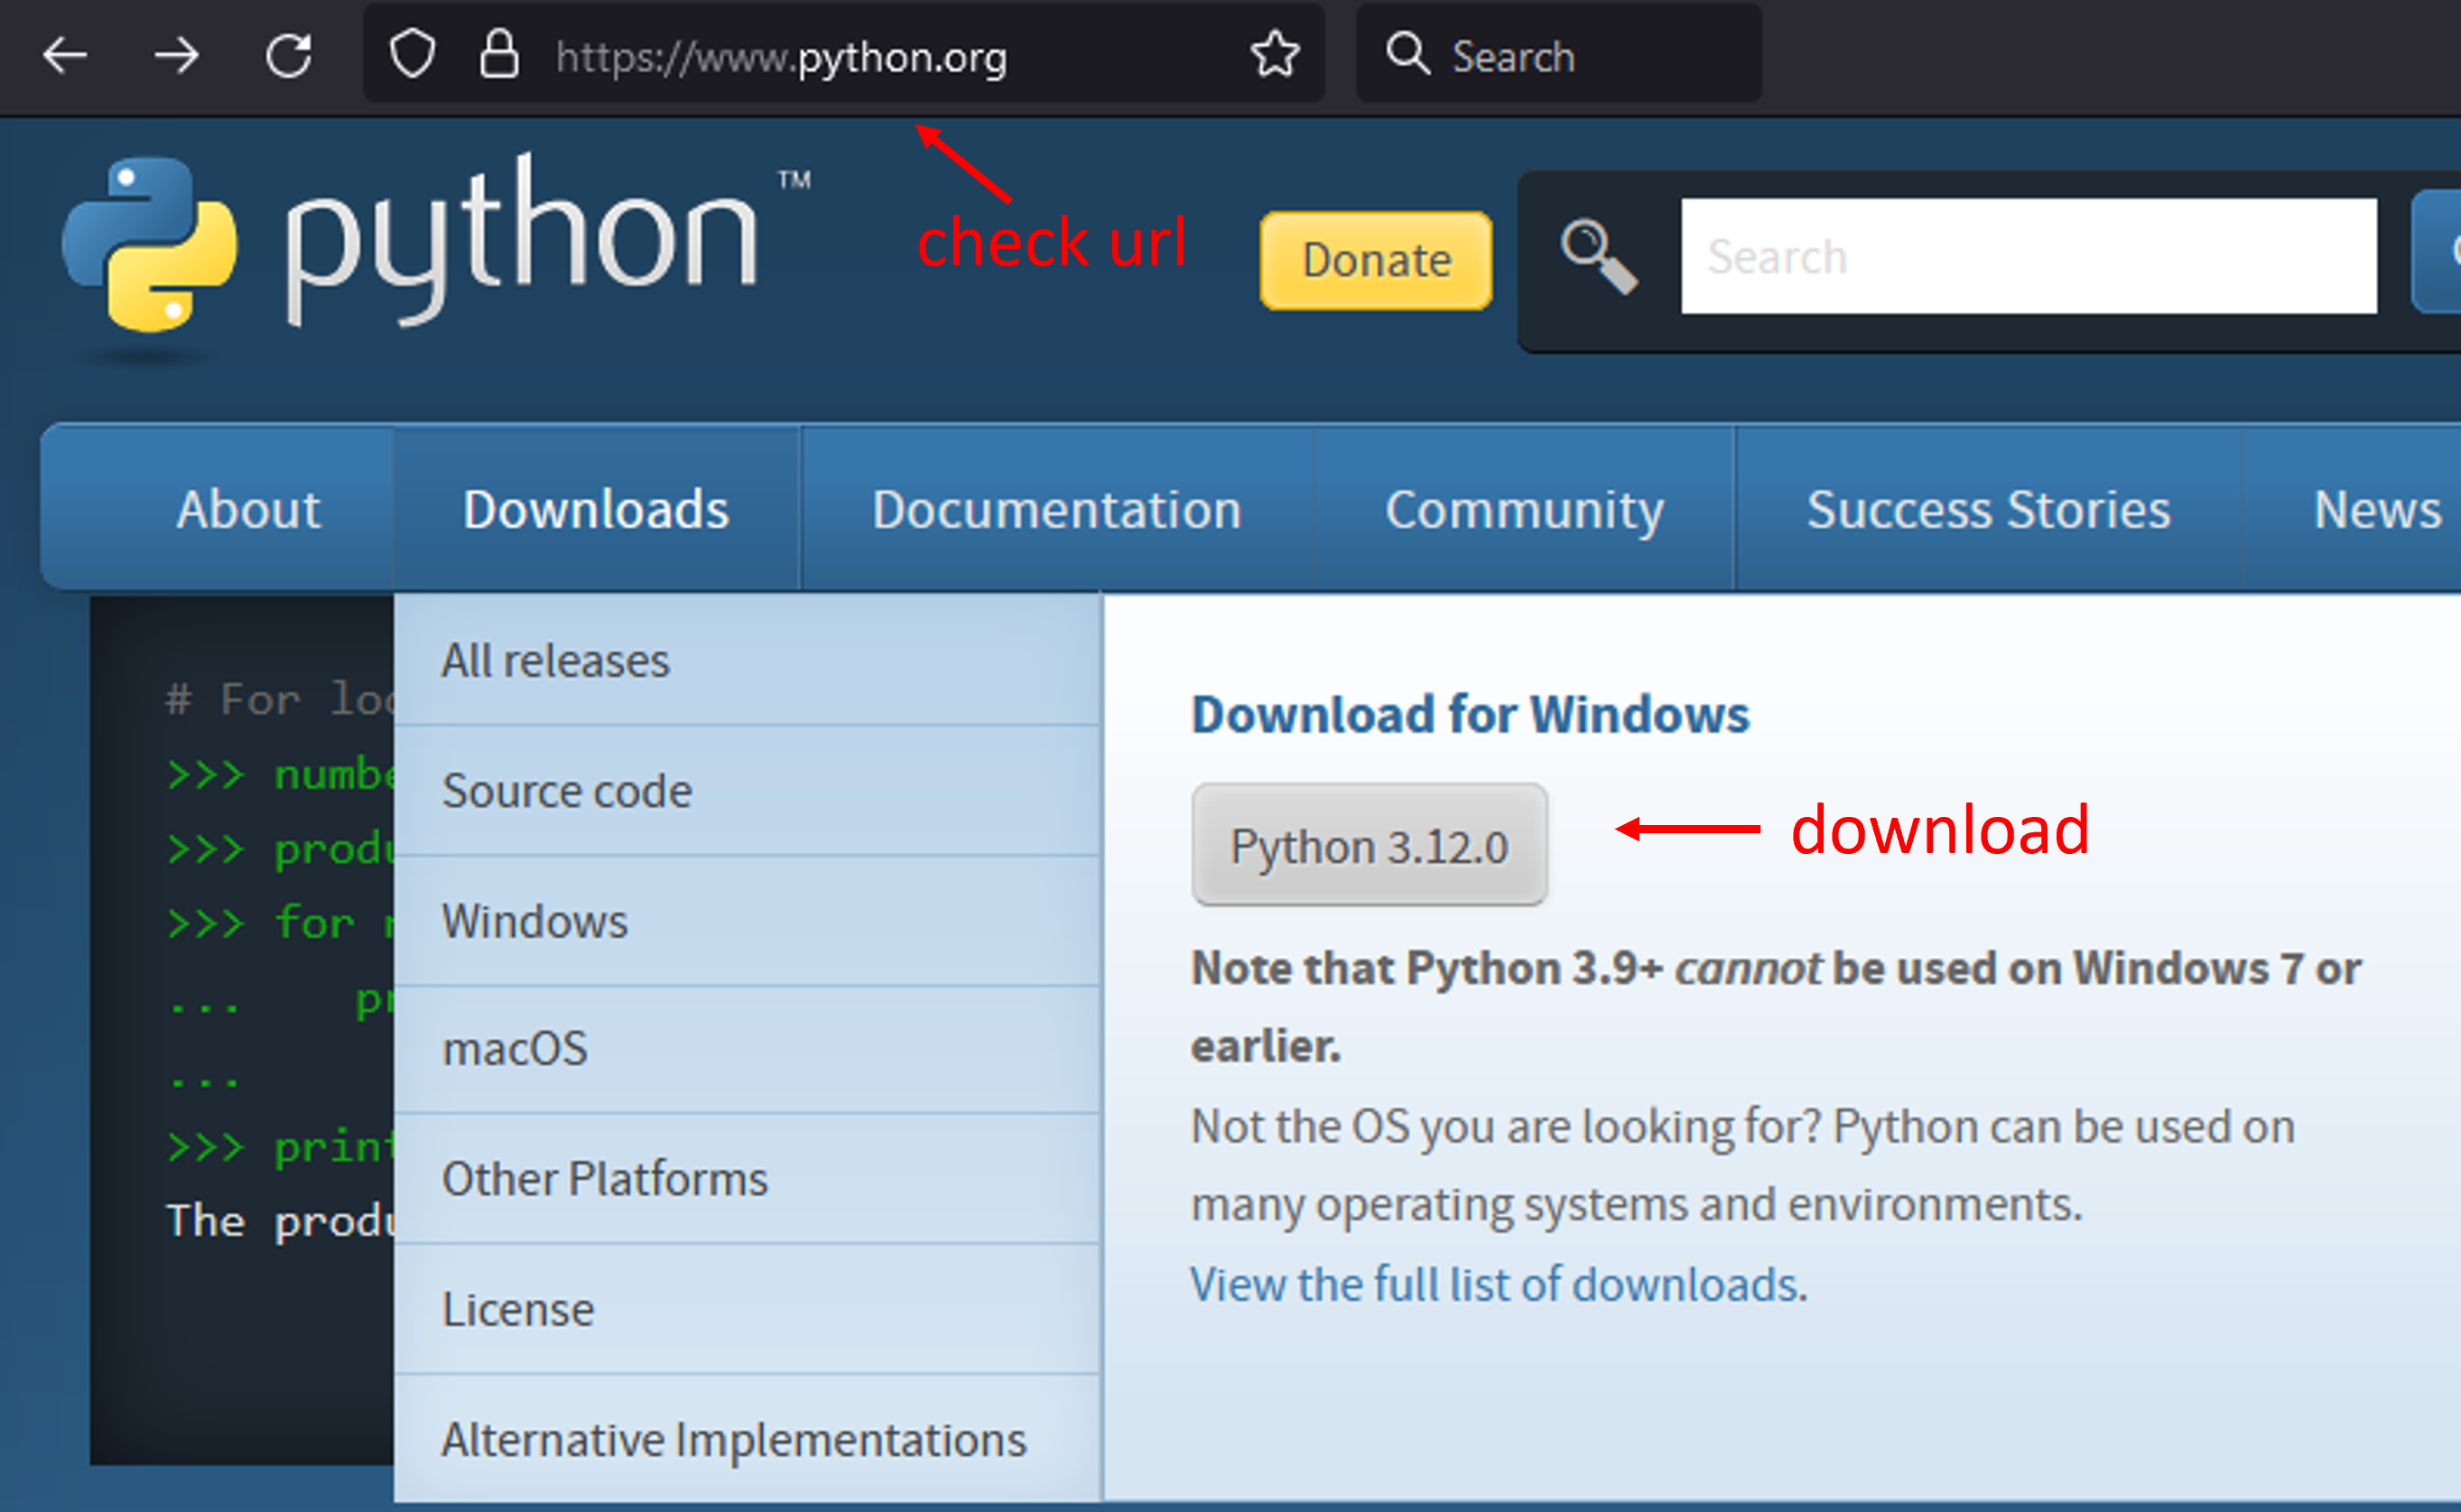
\includegraphics[width=0.8\textwidth]{images/0_python.org.png}
\end{figure}
\end{frame}

\begin{frame}
\frametitle{Setting Up Python 3 in Windows}
While installing, make sure to check ``Add python.exe to PATH''.
\begin{figure}[H]
\centering
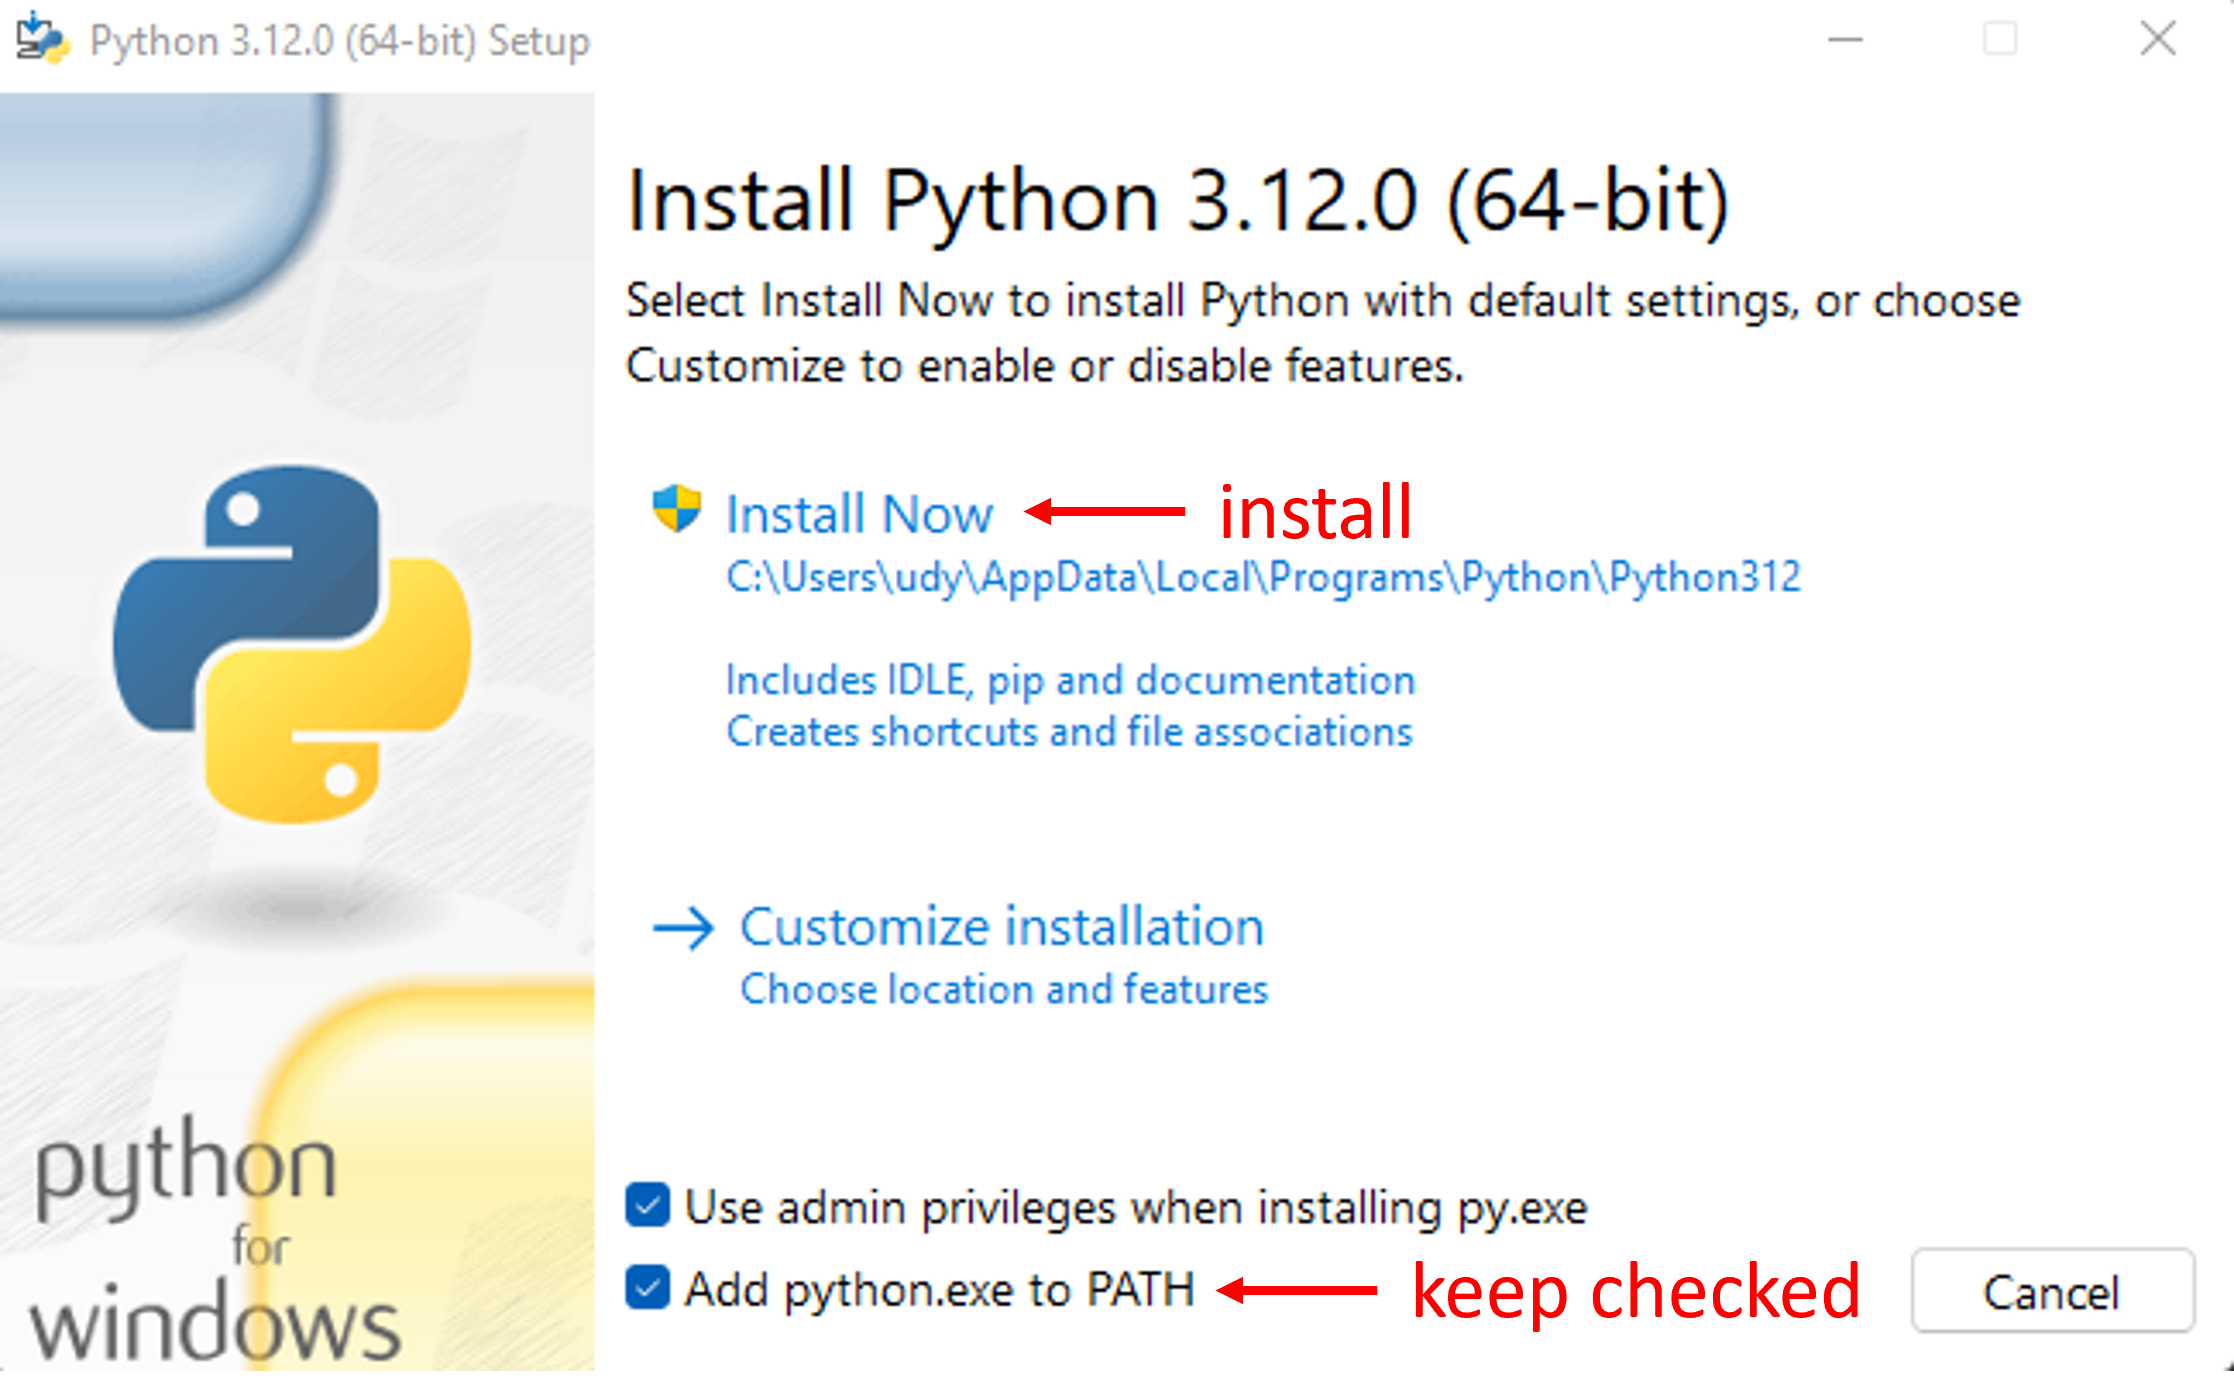
\includegraphics[width=0.8\textwidth]{images/0_windows-setup.png}
\end{figure}
\end{frame}

\begin{frame}
\frametitle{Setting Up Python 3 in Windows}
Additional python packages can be installed using \lstinline{pip} command in Windows command prompt, e.g., \lstinline{pip install numpy}.
\begin{figure}[H]
\centering
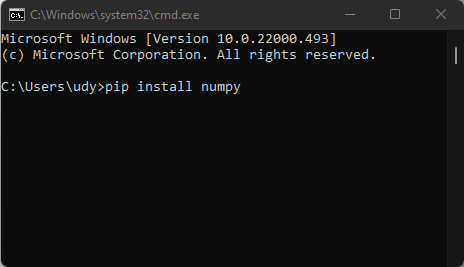
\includegraphics[width=0.8\textwidth]{images/0_windows-pip.png}
\end{figure}
\end{frame}

\begin{frame}
\frametitle{Setting Up Python 3 in Ubuntu}
\begin{enumerate}
\item Python 3 must be pre-installed in new Ubuntu versions, check it by running the command \lstinline{python3 --version} in terminal.
\item If not found, install using the command \lstinline{sudo apt install python3}.
\item Additional python packages can be installed using \lstinline{pip} command in terminal, e.g., \lstinline{pip install numpy}.
\item Recent Ubuntu versions don't allow \lstinline{pip} to easily modify system packages. As a quick workaround, use \lstinline{pip} as \lstinline{pip install numpy --break-system-packages}, which should be fine for some basic usage.
\end{enumerate}
\end{frame}

\begin{frame}
\frametitle{Setting Up Python 3 in Android}
\begin{enumerate}
\item Install \emph{Termux} from F-Droid or Google Play Store, this will act as proxy for Linux terminal.
\item Update packages with command \lstinline{pkg update} in Termux.
\item Install python using \lstinline{pkg install python python-numpy python-pip} in Termux.
\item For now, \lstinline{pip} doesn't work properly in Termux, so only some basic usage is possible.
\end{enumerate}
\end{frame}

\begin{frame}
\frametitle{Editing and Running the code}
\begin{enumerate}
\item In Windows, make an empty file with extension \lstinline{.py}. Right click on this file and open with \textbf{IDLE} editor. To run the code, press \textbf{F5} key.
\item Alternately, I'll suggest using \textbf{Notepad++} in Windows. Python code then can be run from command prompt or powershell using command \lstinline{python mycode.py}.
\item In Ubuntu, make an empty file with extension \lstinline{.py}. You can edit this file using any text editor like \textbf{gedit}, \textbf{vim}, etc. To run the code, run the command \lstinline{python3 mycode.py} from terminal.
\item In Android, you can use \textbf{vim} from \textbf{Termux} to make and edit \lstinline{.py} files. To run the code, run the command \lstinline{python3 mycode.py} from Termux.
\end{enumerate}
\end{frame}

\begin{frame}
\frametitle{Editing and Running the code}
Your setup with \textbf{IDLE} on Windows should look like this:
\begin{figure}[H]
\centering
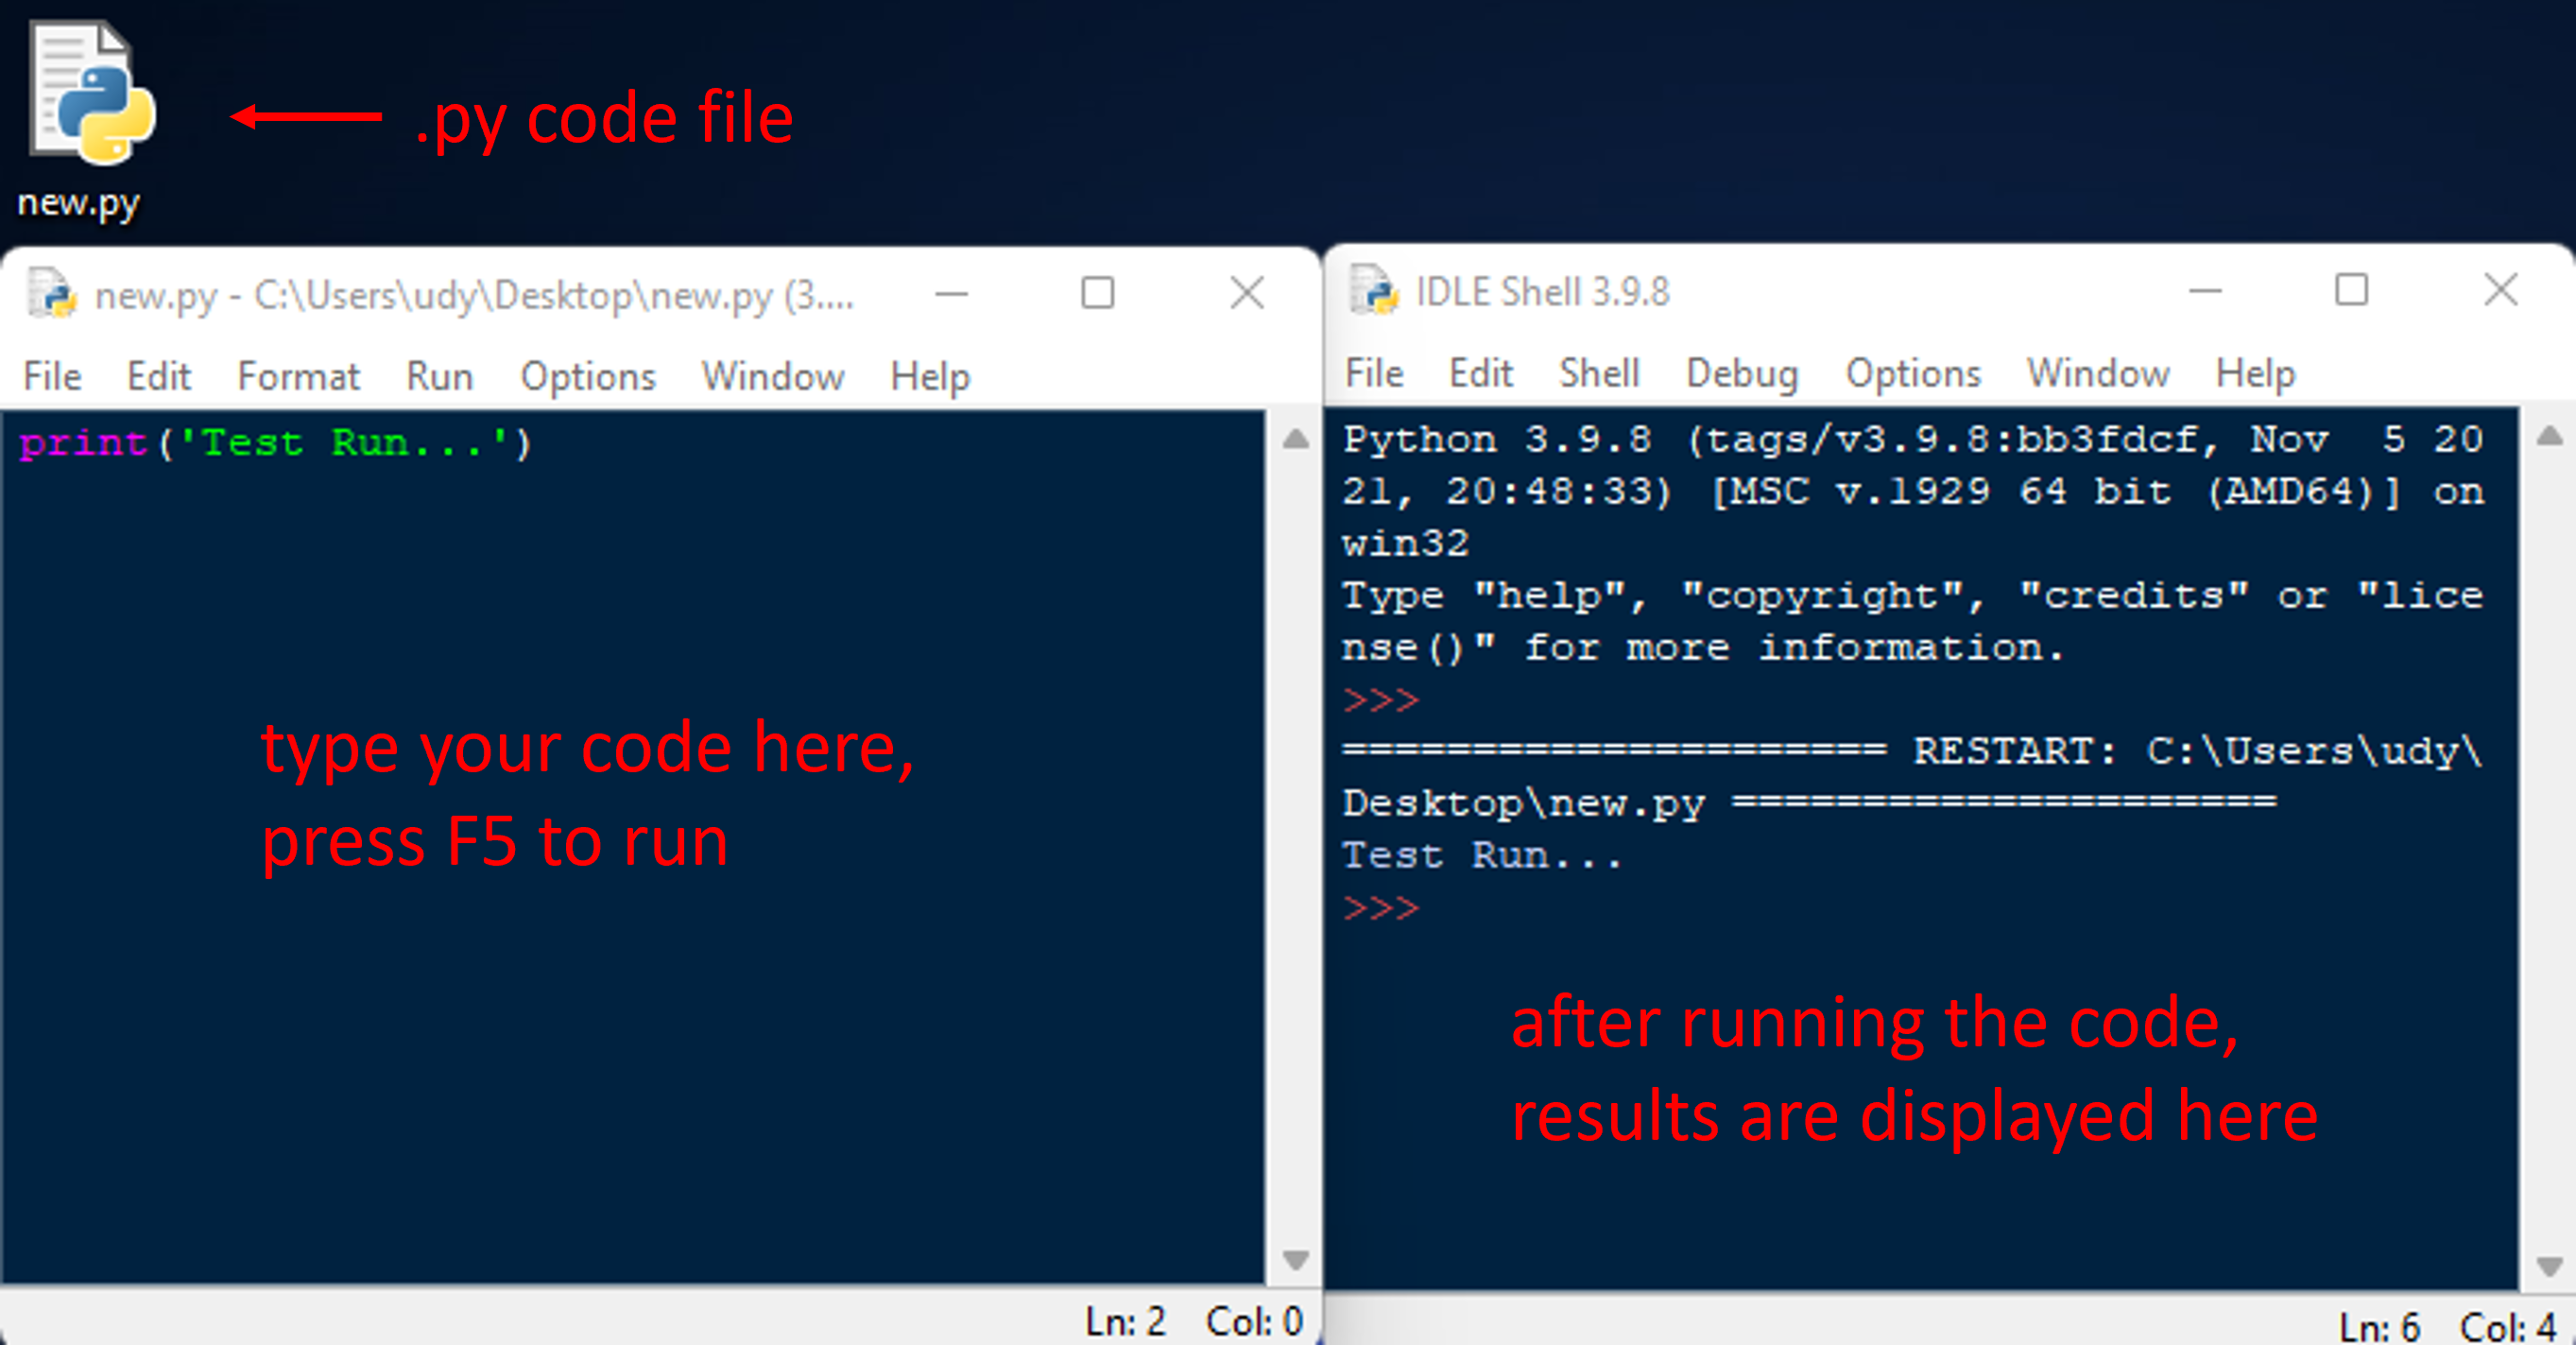
\includegraphics[width=\textwidth]{images/0_windows-idle.png}
\end{figure}
\end{frame}

\begin{frame}
\frametitle{Editing and Running the code}
Your setup with \textbf{Notepad++} on Windows should look like this:
\begin{figure}[H]
\centering
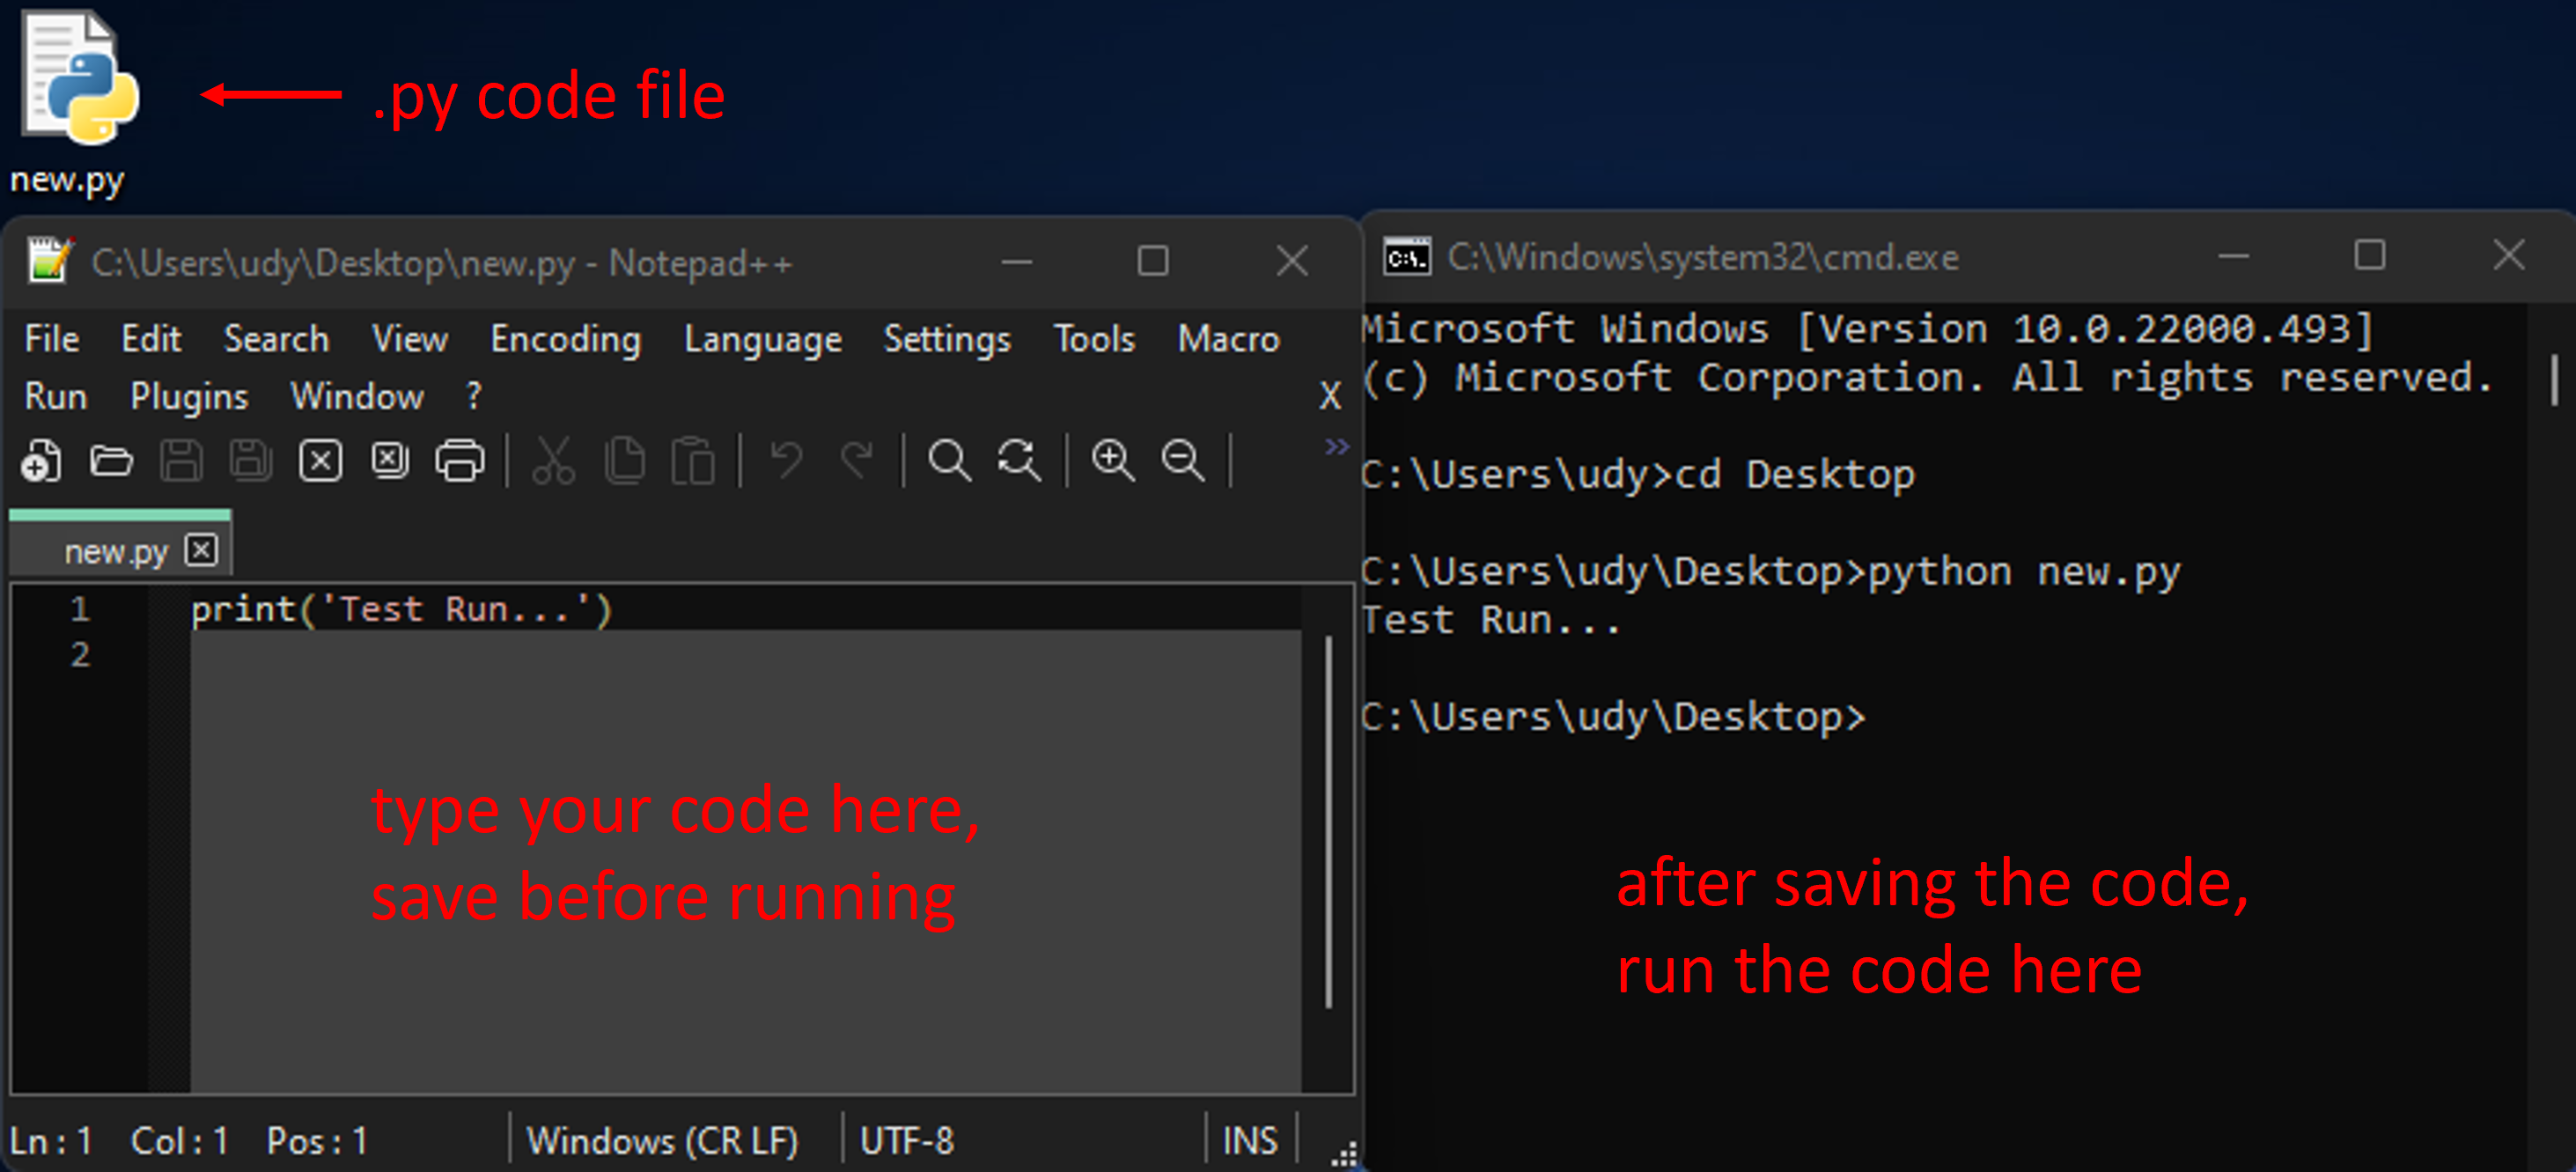
\includegraphics[width=\textwidth]{images/0_windows-notepad++.png}
\end{figure}
\end{frame}

\begin{frame}
\frametitle{Editing and Running the code}
Your setup with \textbf{gedit} on Ubuntu should look like this:
\begin{figure}[H]
\centering
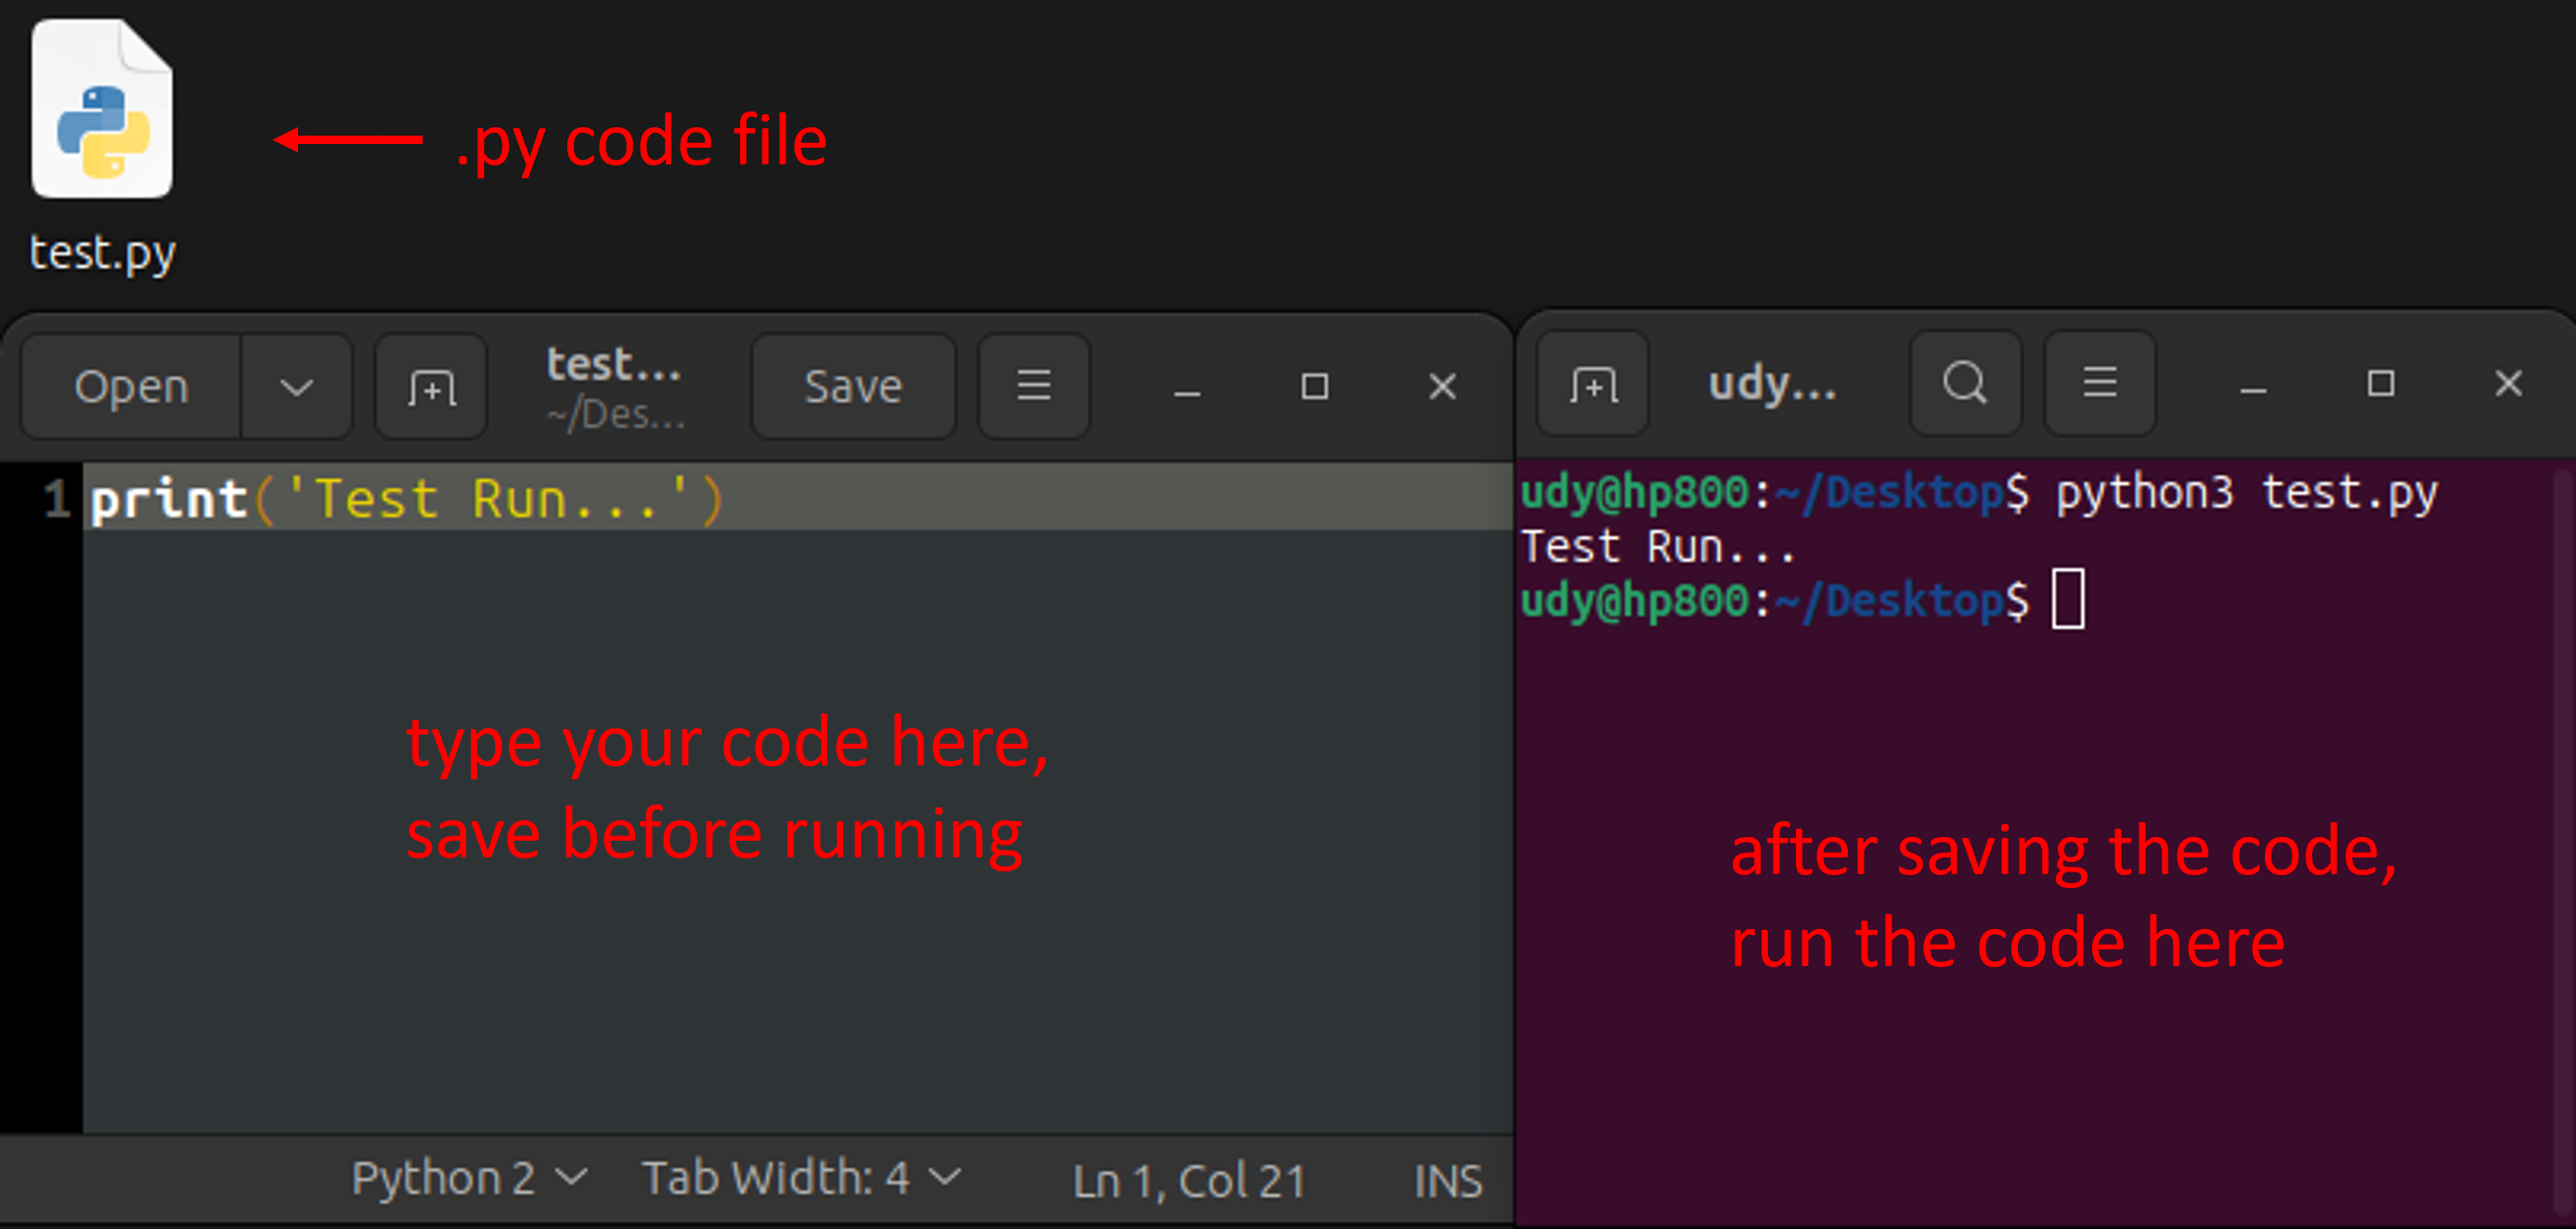
\includegraphics[width=\textwidth]{images/0_ubuntu-gedit.png}
\end{figure}
\end{frame}

\begin{frame}
\frametitle{Editing and Running the code}
Your setup with \textbf{vim} on Android should look like this:
\begin{figure}[H]
\centering
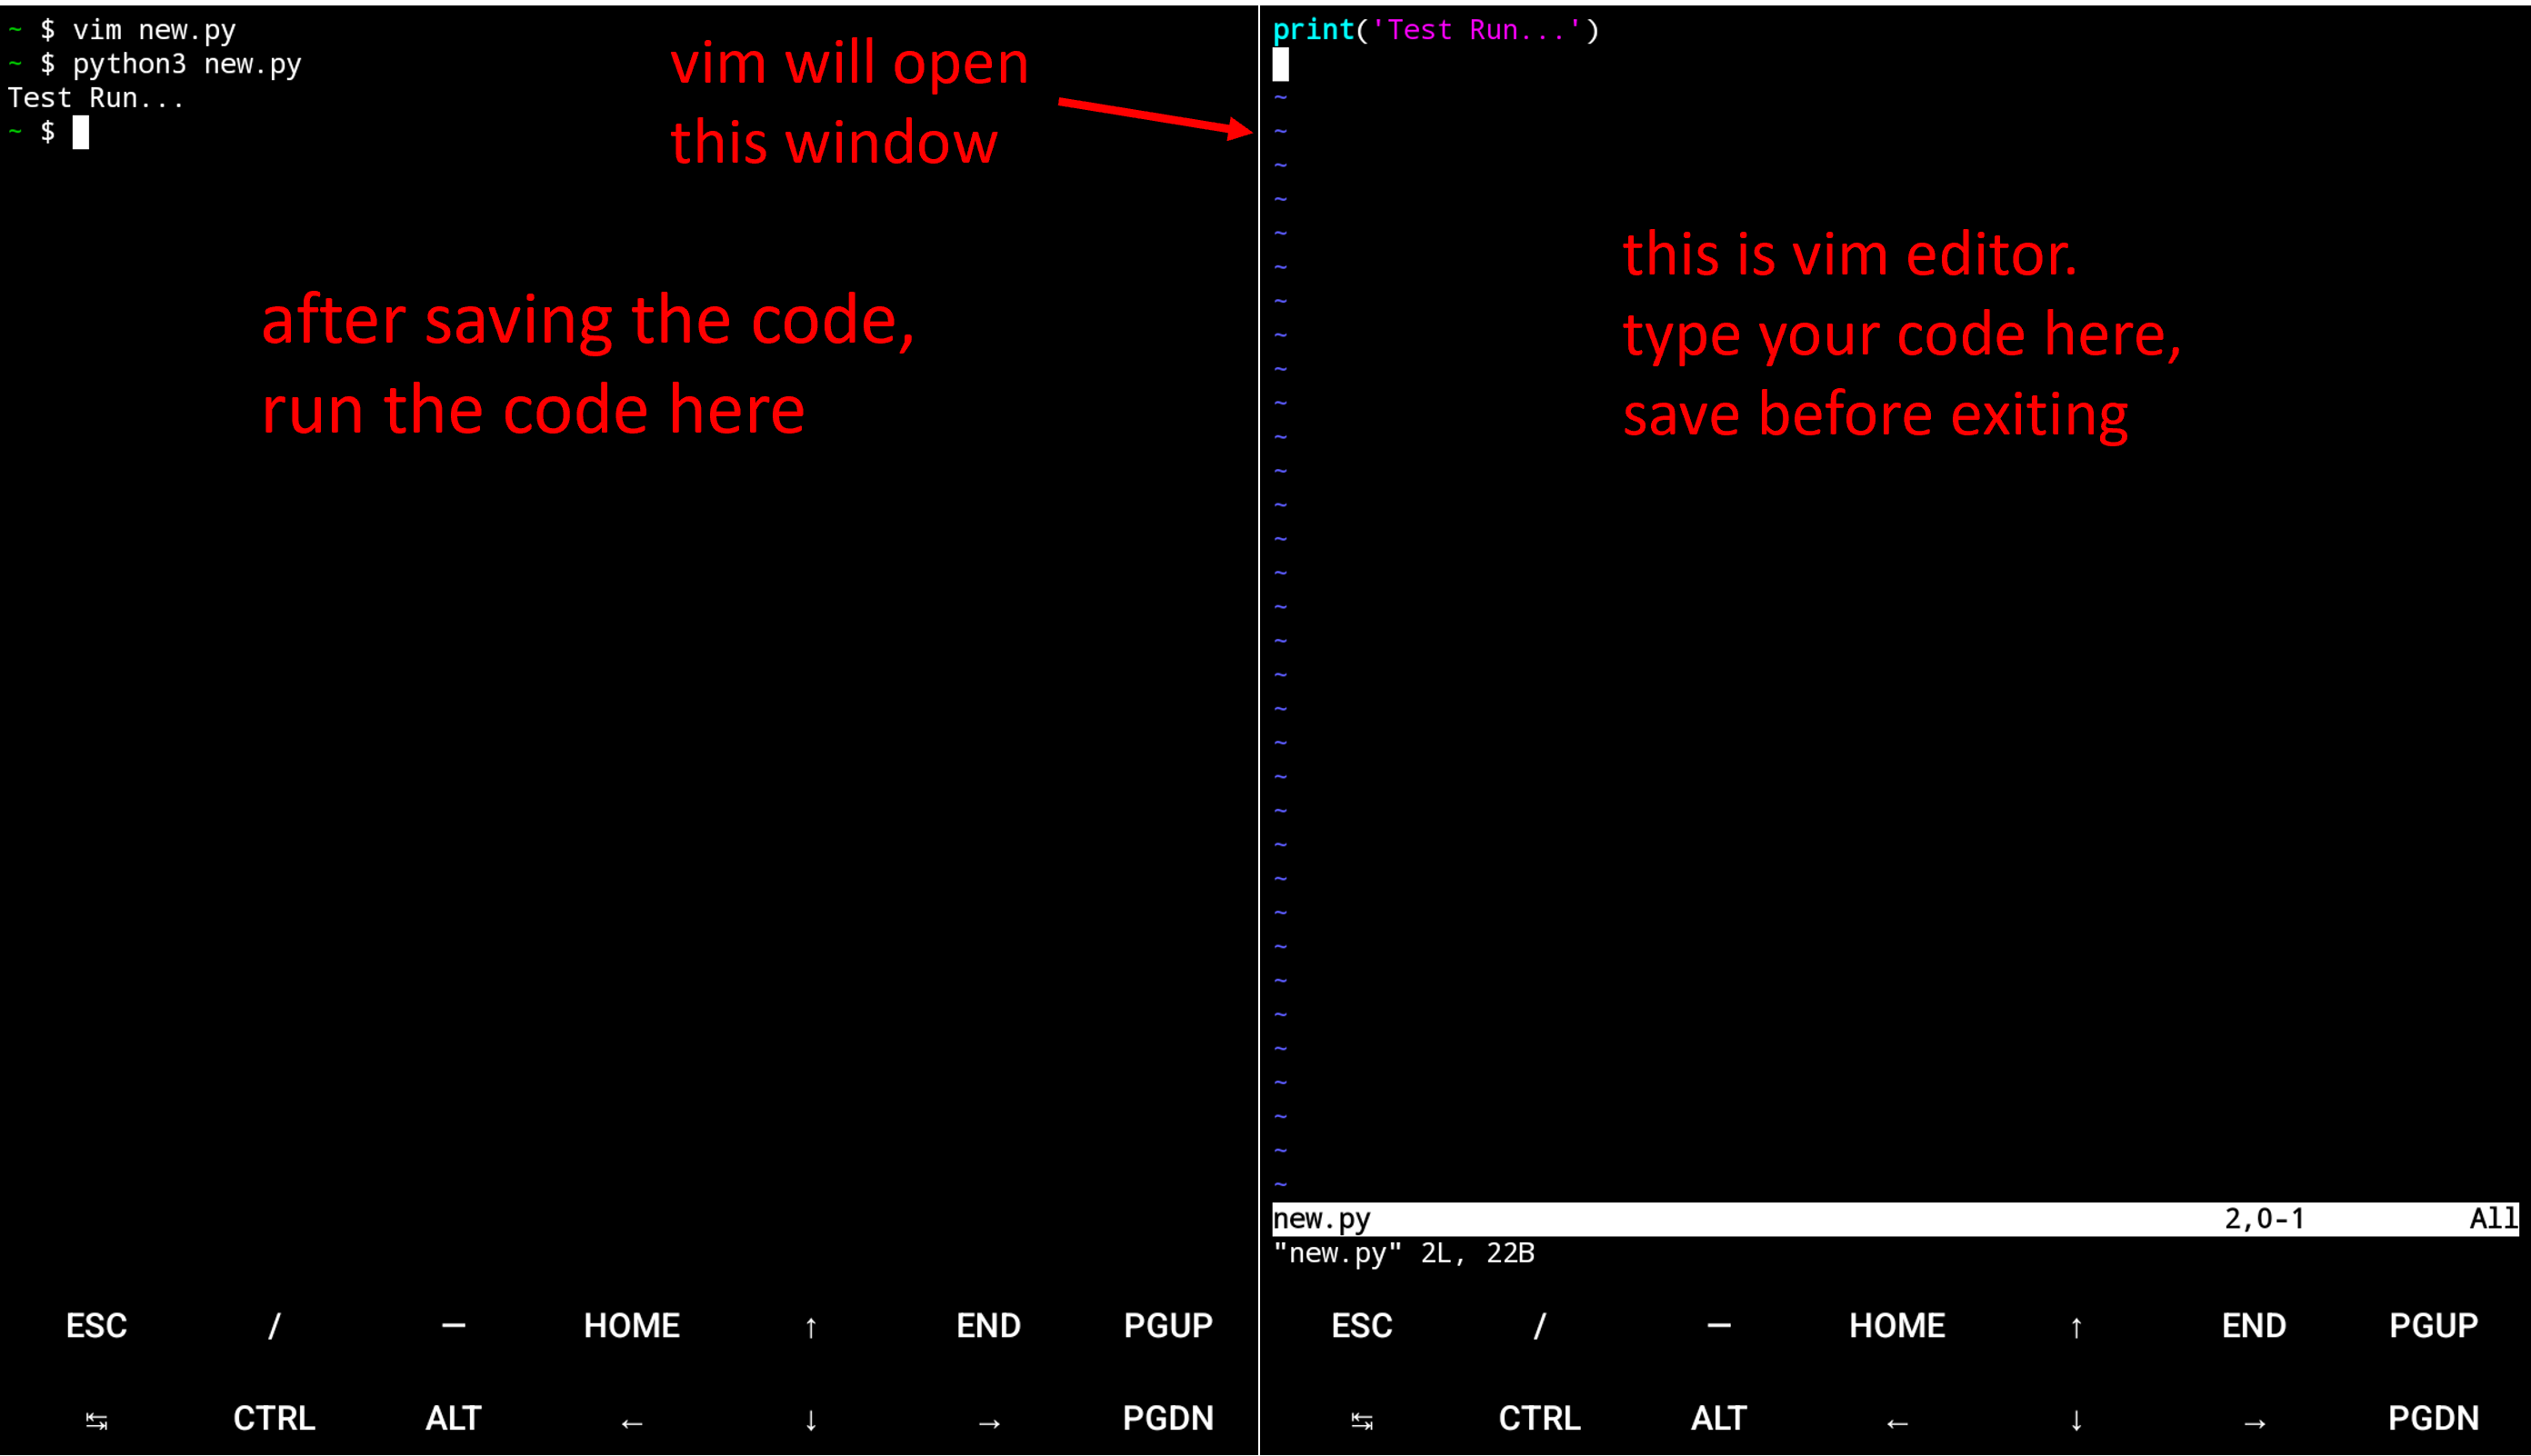
\includegraphics[width=\textwidth]{images/0_android-vim.png}
\end{figure}
\end{frame}

\section{Data Types}

\begin{frame}
\frametitle{Variables}
A \textbf{variable} is a name given to an object, for later referencing.
\begin{figure}[H]
\centering
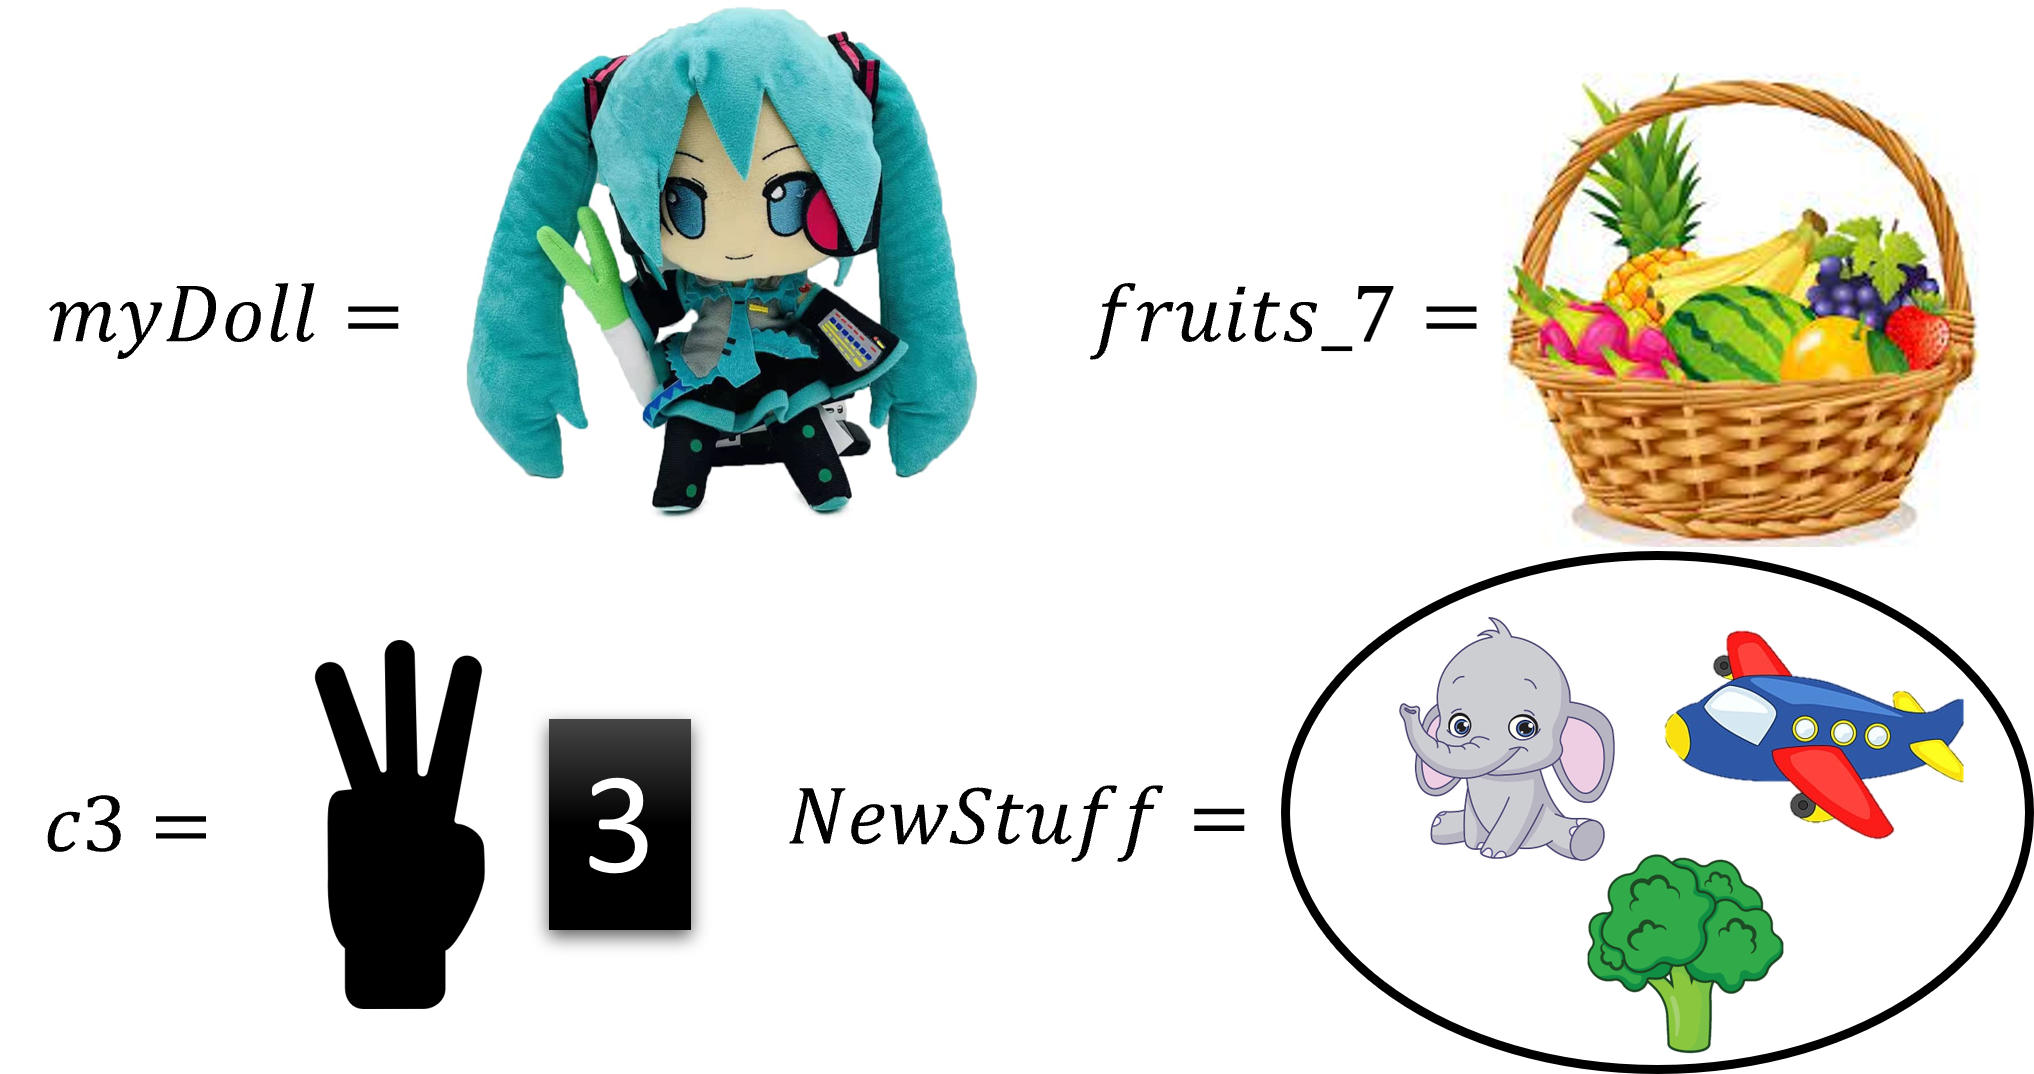
\includegraphics[width=\textwidth]{images/0_variables-examples.png}
\end{figure}
\end{frame}

\begin{frame}[fragile]
\frametitle{Variables}
\begin{enumerate}
\item Variables can contain alphabets \emph{a-z, A-Z}, underscore \emph{\_} and numerals \emph{0-9}.
\item Variable names cannot start with numerals. You should also avoid starting the variable with \emph{\_} for now, because it holds special meaning in Python.
\item Variables are case-sensitive in Python, \pyth{Ab} $\ne$ \pyth{ab}.
\item Variables cannot be Python's keywords (like \pyth{print, and, for, try}, etc.). Find complete list by using the following code:
\begin{python}
import keyword
print(keyword.kwlist)
\end{python}
\end{enumerate}
\end{frame}

\begin{frame}
\frametitle{Data Types}
\textbf{Data Types} refer to the types of objects. Objects are an instance of a \textbf{class}. Some commonly used classes are:
\begin{enumerate}
\item Numerical data types: \lstinline{int}, \lstinline{float}, \lstinline{complex}
\item Words data type: \lstinline{str}
\item Logical data type: \lstinline{bool}
\item Collection data types: \lstinline{list}, \lstinline{tuple}, \lstinline{dict}
\end{enumerate}
\end{frame}

\begin{frame}[fragile]
\frametitle{\pyth{type} command}
Class of a variable can be checked using \pyth{type} command. For example, the following code
\begin{python}
x = 1
print(type(x))
\end{python}
should print \lstinline{<class `int'>}. And the following code
\begin{python}
t_0 = (1, 'a', 2.3)
print(type(t_0))
\end{python}
should print \lstinline{<class `tuple'>}.
\end{frame}

\begin{frame}[fragile]
\frametitle{\lstinline{int} Data Type}
\begin{enumerate}
\item All integers belong this class.
\item Unconventionally, Python stores \lstinline{int} with as much required space as needed. But large values will require more storage and reduce code's efficiency.
\item Examples of \lstinline{int} are \pyth{2}, \pyth{-714}, \pyth{0}.
\end{enumerate}
\end{frame}

\begin{frame}[fragile]
\frametitle{\lstinline{float} Data Type}
\begin{enumerate}
\item All real numbers belong to this class.
\item Python defaults to 64-bit storage for \lstinline{float}, unless forcefully specified or the machine doesn't support. You can assume accuracy of about $15$ digits after decimal.
\item Python uses floating-point representation. Its range in a machine can be found using the command \pyth{sys.float_info}.
\item Examples of \lstinline{float} are \pyth{0.0}, \pyth{-1.0}, \pyth{0.0052351}, \pyth{6.3e8}, \pyth{-0.03e-5}.
\end{enumerate}
\end{frame}

\begin{frame}[fragile]
\frametitle{\lstinline{complex} Data Type}
\begin{enumerate}
\item All complex numbers belong to this class.
\item Similar to \lstinline{float}, \lstinline{complex} uses 64-bit precision for both real and imaginary part.
\item The imaginary part in a complex number is written as \pyth{j} like \pyth{1+2j}. Or the \pyth{complex} command can be used like \pyth{complex(1,2)}.
\item If \pyth{z} is a complex number, access its real part with \pyth{z.real} and imaginary part with \pyth{z.imag}.
\item Examples of \lstinline{complex} are \pyth{1+1j}, \pyth{0.4-3.9j}, \pyth{2.3e3j}, \pyth{0j}.
\item For operations involving complex numbers, \pyth{cmath} library is encouraged to be used.
\end{enumerate}
\end{frame}

\begin{frame}[fragile]
\frametitle{\lstinline{str} Data Type}
\begin{enumerate}
\item All strings and characters belong to this class.
\item Strings can be written using single quotes \pyth{'...'} or double quotes \pyth{"..."}.
\item Strings can be also be written using triple single/double quotes \pyth{'''...'''} or \pyth{"""..."""}. This facilitates writing large texts like paragraphs or commenting large section of code.
\item Any variable can be converted to \lstinline{str} type using \pyth{str} command, if the variable supports it.
\end{enumerate}
\end{frame}

\begin{frame}[fragile]
\frametitle{\lstinline{bool} Data Type}
\begin{enumerate}
\item This class has only 2 elements \pyth{True} and \pyth{False}.
\item These values inherently support all boolean operations, discussed later.
\item Any variable can be converted to \lstinline{bool} type using \pyth{bool} command, if the variable supports it.
\item It is worth noting that non-zero numbers and non-empty arrays convert to \pyth{True}, otherwise they convert to \pyth{False}.
\end{enumerate}
\end{frame}

\begin{frame}[fragile]
\frametitle{\lstinline{list} Data Type}
\begin{enumerate}
\item \lstinline{list} is an ordered and mutable collection of different objects.
\item It is defined and represented with square brackets \pyth{[...]}.
\item Examples of \lstinline{list} are \pyth{[]}, \pyth{[71, -99, 71, 4]}, \pyth{[3, 3.0, 'three']}, \pyth{[3, ['Alpha', -1], True]}.
\item Length of a \lstinline{list} can be found using \pyth{len} command. For example, \pyth{len([])} will print \pyth{0} and \pyth{len([[1.7, -3.8], 0, [], 'xyz'])} will print \pyth{4}.
\item A particular \pyth{i}$^{th}$ element of a \lstinline{list} \pyth{x} can be accessed as \pyth{x[i]}. For example, if \pyth{z=[-3, 4, 7.8]}, then \pyth{z[1]} will refer to \pyth{4} (remember that Python indexing starts from $0$).
\end{enumerate}
\end{frame}

\begin{frame}[fragile]
\frametitle{\lstinline{tuple} Data Type}
\begin{enumerate}
\item \lstinline{tuple} is an ordered and immutable collection of different objects.
\item It is defined and represented with circular brackets \pyth{(...)}.
\item Examples of \lstinline{tuple} are \pyth{()}, \pyth{(71, )}, \pyth{(3, 3.0, 'three')}, \pyth{(3, ['Alpha', -1], True, 3)}.
\item Finding length and indexing work same as \lstinline{list}.
\end{enumerate}
\end{frame}

\begin{frame}[fragile]
\frametitle{\lstinline{dict} Data Type}
\begin{enumerate}
\item \lstinline{dict} or dictionary is a mutable \emph{key:value} collection of data.
\item \emph{Value} can be any data type but \emph{key} has restrictions like they should be unique and immutable. Prefer keys to be numbers, \lstinline{str}, \lstinline{tuple}.
\item It is defined and represented with curly brackets \{ \}.
\item Examples of \lstinline{dict} are:
\begin{python}
{}, {0:'ax', 1:'by', 2:'cz'},
{'a':4, 4.9:'qko', 'd':[4,6,9], 'e0':()}
\end{python}
\item Finding length works same as \lstinline{list}. For accessing a value of a \lstinline{dict}, its key must be used as index. For example if \pyth{d} is the last dict above, then \pyth{d[4.9]} will return \pyth{'qko'}.
\end{enumerate}
\end{frame}

\section{Operators}

\begin{frame}
\frametitle{Operators}
An \textbf{operator} performs an operation on one or more objects to produce one or more objects.
\begin{figure}[H]
\centering
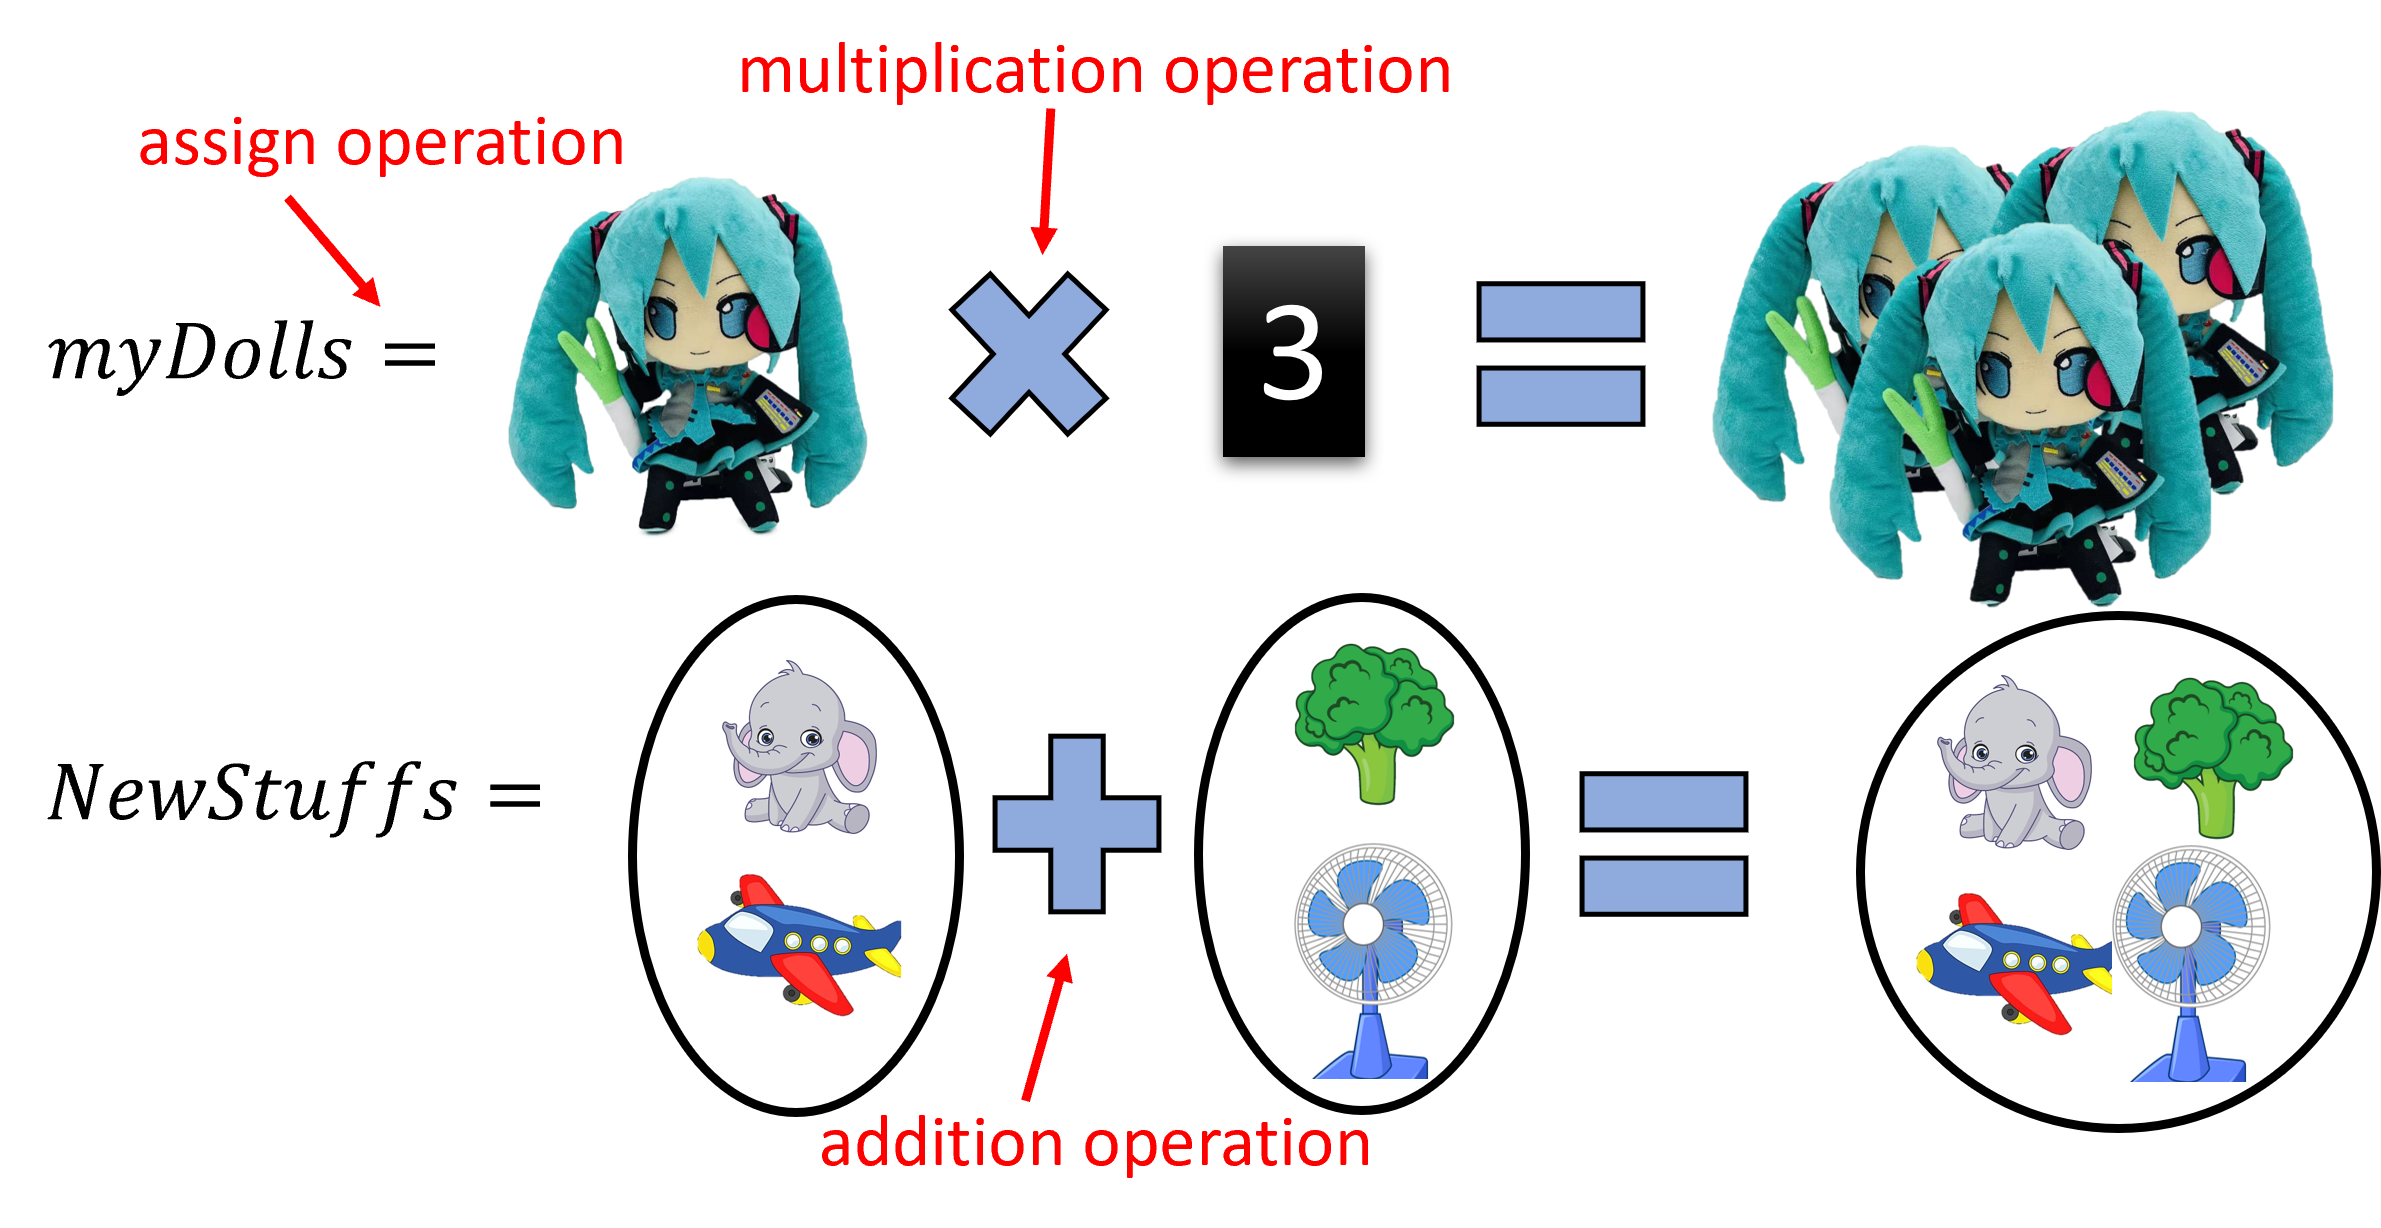
\includegraphics[width=\textwidth]{images/0_operators-examples.png}
\end{figure}
\end{frame}

\begin{frame}[fragile]
\frametitle{Arithmetic Operators}
\begin{enumerate}
\item Addition \pyth{+}, adds numbers. Also works on \lstinline{str}, \lstinline{list}, \lstinline{tuple} by joining them.
\item Subtraction \pyth{-}, subtracts numbers.
\item Multiplication \pyth{*}, multiplies numbers. Also works on \lstinline{str}, \lstinline{list}, \lstinline{tuple} if one argument is an \lstinline{int}, for example, \pyth{[2, 3] * 2} will return \pyth{[2, 3, 2, 3]} and \pyth{4 * 'g'} will return \pyth{'gggg'}.
\item Division \pyth{/}, divides numbers.
\item Floor Division \pyth{//}, divides integers or real numbers and takes \emph{floor} or \emph{greatest integer function}.
\item Remainder \pyth{%}, returns remainder of division operation.
\item Power \pyth{**}, performs power operation for numbers.
\end{enumerate}
\end{frame}

\begin{frame}[fragile]
\frametitle{Bitwise Operators}
These operators work on \lstinline{int}. To understand them, use binary representation.
\begin{enumerate}
\item AND \pyth{&}, \pyth{23 & 14} will return \pyth{6}.
\item OR \pyth{|}, \pyth{23 | 14} will return \pyth{31}.
\item XOR \pyth{^}, \pyth{23 ^ 14} will return \pyth{25}.
\item NOT $\sim$, $\sim$\pyth{23} will return \pyth{-24}.
\item LEFT SHIFT \pyth{<<}, \pyth{23 << 2} will return \pyth{92}.
\item RIGHT SHIFT \pyth{>>}, \pyth{23 >> 2} will return \pyth{5}.
\end{enumerate}
\end{frame}

\begin{frame}[fragile]
\frametitle{Logical Operators}
These operators work on \lstinline{bool}. Note how they differ from bitwise operators.
\begin{enumerate}
\item \pyth{and}, \pyth{False and True} will return \pyth{False}.
\item \pyth{or}, \pyth{False or True} will return \pyth{True}.
\item \pyth{not}, \pyth{not False} will return \pyth{True}.
\end{enumerate}
\end{frame}

\begin{frame}[fragile]
\frametitle{Assignment Operators}
\pyth{=}, used to assign an object to a variable. \\
The other assignment operators are derivatives of arithmetic and bitwise operators. They are \pyth{+=, -=, *=, /=, //=, %=, **=, &=, |=, ^=, <<=, >>=} \\
For example, if \pyth{x = 5}, then the command \pyth{x += 2.3} with store value \pyth {7.3} to variable \pyth{x}.
\end{frame}

\begin{frame}[fragile]
\frametitle{Comparison Operators}
These operators work on numbers. They can also work on \lstinline{list} and \lstinline{tuple} following a Lexicographic order. They always return \lstinline{bool} value \pyth{True} or \pyth{False}.
\begin{enumerate}
\item Equal To \pyth{==}, \pyth{0 == 0.0} will return \pyth{True}.
\item Not Equal To \pyth{!=}, \pyth{0 != 0.0} will return \pyth{False}.
\item Less Than \pyth{<}, \pyth{0 < 0.0} will return \pyth{False}.
\item Less Than Equal To \pyth{<=}, \pyth{0 <= 0.0} will return \pyth{True}.
\item Greater Than \pyth{>}, \pyth{0 > 0.0} will return \pyth{False}.
\item Greater Than Equal To \pyth{>=}, \pyth{0 >= 0.0} will return \pyth{True}.
\end{enumerate}
\end{frame}

\begin{frame}[fragile]
\frametitle{Special Operators}
Operator \pyth{is} requires object's class to match as well. Operator \pyth{in} checks if the object exists in a sequence or not.
\begin{enumerate}
\item \pyth{is}, \pyth{0 is 0.0} will return \pyth{False}.
\item \pyth{is not}, \pyth{0 is not 0.0} will return \pyth{True}.
\item \pyth{in}, \pyth{0 in [0.0, 1, 2j]} will return \pyth{True}.
\item \pyth{not in}, \pyth{0 not in [0.0, 1, 2j]} will return \pyth{False}.
\end{enumerate}
\end{frame}

\begin{frame}[fragile]
\frametitle{Operators Precedence}
If multiple operators are used in an expression, first parentheses are resolved separately. In an expression without parentheses operations are resolved in this priority:

\begin{enumerate}
\item \pyth{**}
\item \pyth{+x, -x, } $\sim$\pyth{x}
\item \pyth{*, /, //, %}
\item \pyth{+, -}
\item \pyth{<<, >>}
\item \pyth{&}
\item \pyth{^}
\item \pyth{|}
\asuivre
\end{enumerate}
\end{frame}

\begin{frame}[fragile]
\frametitle{Operators Precedence}
\begin{enumerate}
\suite
\item \pyth{==, !=, <=, >=, <, >, is, is not, in, not in}
\item \pyth{not}
\item \pyth{and}
\item \pyth{or}
\end{enumerate}
To avoid confusions, always prefer to use parentheses. So instead of writing \\
\pyth{2 ** 3 > -4 + 9 and not 4 / 2 is 2} \\
write \\
\pyth{((2 ** 3) > (-4 + 9)) and (not ((4 / 2) is 2))}
\end{frame}

\section{Writing Style}

\begin{frame}
\frametitle{Code Writing Conventions}
\begin{enumerate}
\item Python Enhancement Proposal (PEP) 8 suggests conventions of writing a Python code.
\item These are not necessary but highly recommended to write a consistent readable code.
\item You can adapt different styles but remain consistent.
\item Don't use \emph{tabs} in Python code, they could work for you but often cause problems.
\begin{itemize}
\item In \textbf{Notepad++}, go to Settings $\rightarrow$ Preferences $\rightarrow$ Language $\rightarrow$ Tab Settings and check \emph{Replace by space}.
\item In \textbf{gedit}, go to Edit $\rightarrow$ Preferences $\rightarrow$ Editor and check \emph{Insert spaces instead of tabs}.
\end{itemize}
\item Python code must be UTF-8 encoded. Prefer simple English as much possible.
\item Try running the code \pyth{import this}.
\end{enumerate}
\end{frame}

\begin{frame}
\frametitle{Indentation}
\begin{enumerate}
\item Consistent indentation is important in Python unlike most other programming languages. This will be clear when loops and functions will be discussed.
\item \textbf{4 spaces} are recommeded for indentation.
\end{enumerate}
\begin{figure}[H]
\centering
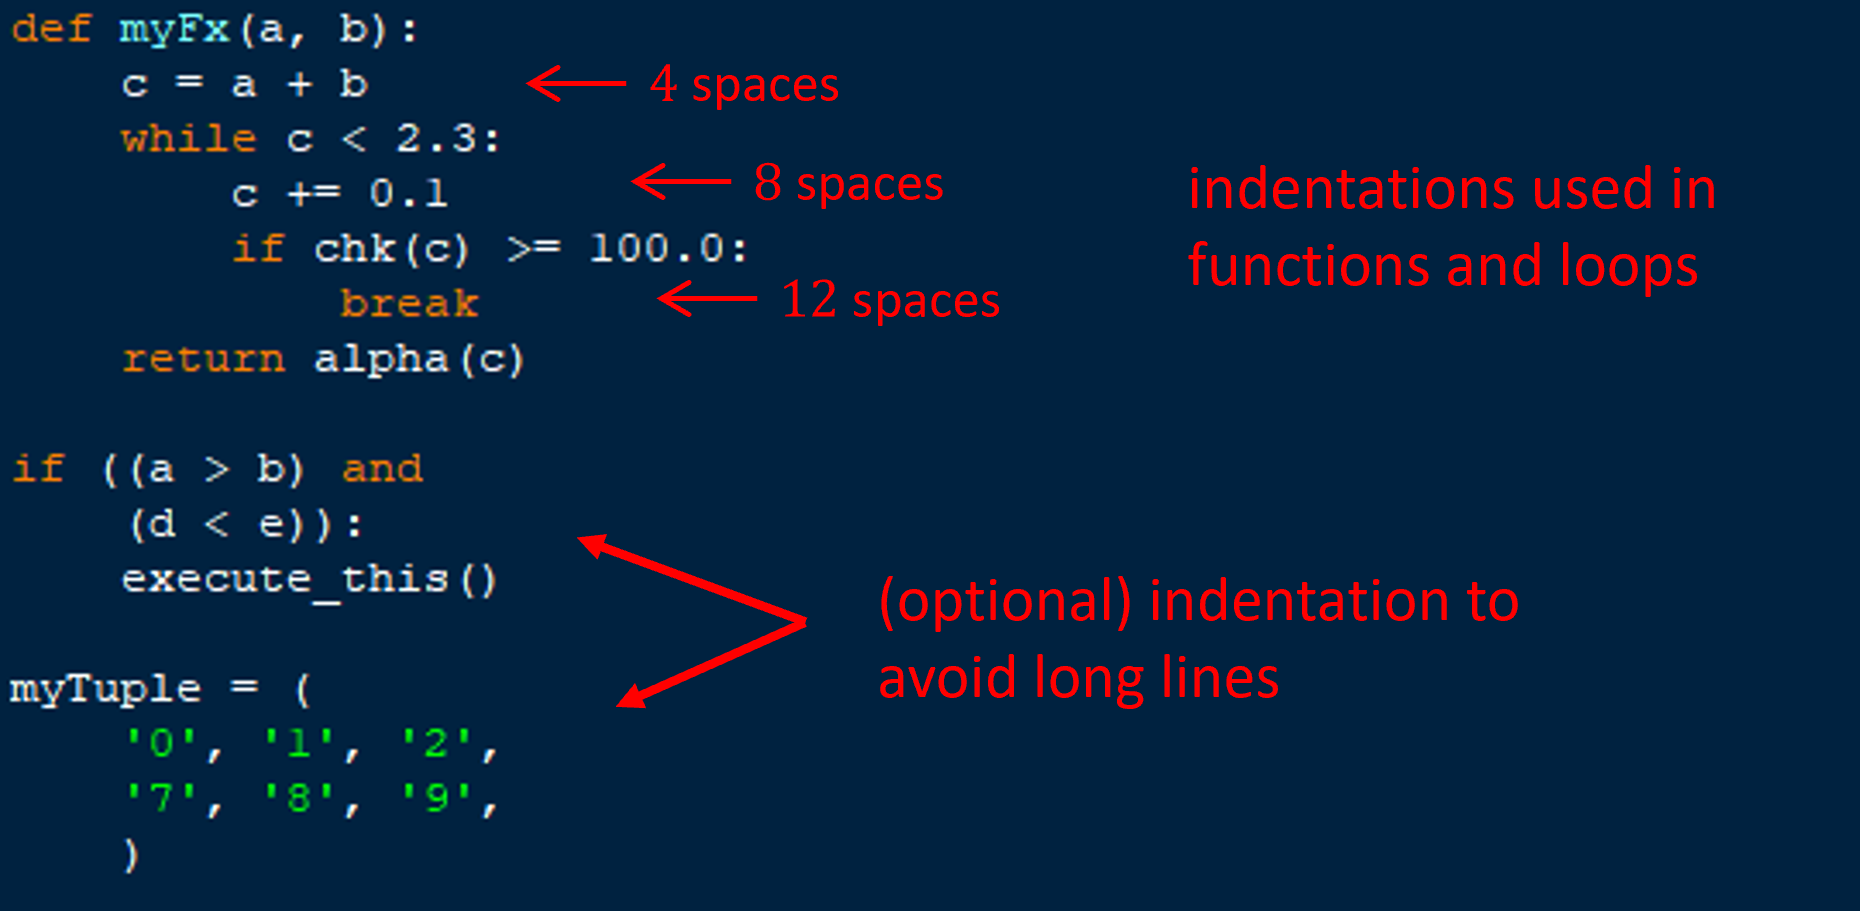
\includegraphics[width=\textwidth]{images/0_indentation.png}
\end{figure}
\end{frame}

\begin{frame}[fragile]
\frametitle{Long Lines}
\begin{enumerate}
\item A maximum length of 79 characters is recommended for code and 72 characters for long text blocks or comments. I'll suggest to not be very strict with this but try to keep lines short.
\item An expression can be broken in multiple lines to keep lines short. For example, instead of \pyth{y = (x ** 2 - 3 * z * x) / (5 * x * z - z ** 2)}, one can also write:
\begin{python}
y = (x ** 2 - 3 * z * x)
y = y / (5 * x * z - z ** 2)
\end{python}
\item A large line can also be written in multiple lines as shown in previous slide.
\end{enumerate}
\end{frame}

\begin{frame}[fragile]
\frametitle{Blank Lines and Imports}
\begin{enumerate}
\item Prefer to leave 2 blank lines above and below \emph{class} definitions and one blank line for \emph{functions} defined within. One blank line can be left to show separate sections of code.
\item Prefer to import libraries in multiple lines instead of single line.
\begin{python}
# Prefer
import os
import sys
from math import sqrt, log

# Avoid
import os, sys
\end{python}
\end{enumerate}
\end{frame}

\begin{frame}[fragile]
\frametitle{Spacing}
Prefer to leave one space before and after each operator, unless you're trying to group them.
\begin{python}
# Prefer
k = k + 1
rho += 1
h2 = b*b + p*p

# Avoid
k=k +1
rho +=1
h2 = b * b + p * p
\end{python}
\end{frame}

\begin{frame}[fragile]
\frametitle{Spacing}
Only single space after comma, semicolon, colon.
\begin{python}
# Prefer
spam(ham[1], {eggs: 2})
foo = (0,)
if x == 4: print(x, y); x, y = y, x

# Avoid
spam( ham[ 1 ], { eggs: 2 } )
foo = (0, )
if x == 4 : print(x , y) ; x , y = y , x
\end{python}
\end{frame}

\begin{frame}[fragile]
\frametitle{Spacing}
In index slicing, colons must stick to variables, unless there are operations or function calls.
\begin{python}
# Prefer
ham[1:9], ham[1:9:3], ham[:9:3], ham[1::3]
ham[: upper_fn(x) : step_fn(x)], ham[:: step_fn(x)]
ham[lower+offset : upper+offset]
ham[lower + offset : upper + offset]

# Avoid
ham[lower + offset:upper + offset]
ham[1: 9], ham[1 :9], ham[1:9 :3]
ham[lower : : step]
\end{python}
\end{frame}

\begin{frame}[fragile]
\frametitle{Spacing}
Brackets should tend to stick to what they are related to.
\begin{python}
# Prefer
spam(1)
dct['key'] = lst[index]
abc = {1: 'one', 2: 'two', 3: 'three'}

# Avoid
spam (1)
dct ['key'] = lst [index]
abc = { 1: 'one', 2: 'two', 3: 'three' }
\end{python}
\end{frame}

\begin{frame}[fragile]
\frametitle{Docstrings}
End single-line docstring in same line but multi-line docstring in next line.
\begin{python}
# Prefer
"""This is a docstring or documentation string

Technically this is a string but if not used in
an expression, Python won't do anything with
this and it'll act like a comment.
"""
"""Single line docstring should end in same line"""

# Avoid
"""A multi-line docstring...
... for example """
"""Single line docstring should end in same line
"""
\end{python}
\end{frame}

\section{Your First Codes}

\begin{frame}
\frametitle{Sample Code}
A simple Python code could look like this:
\begin{figure}[H]
\centering
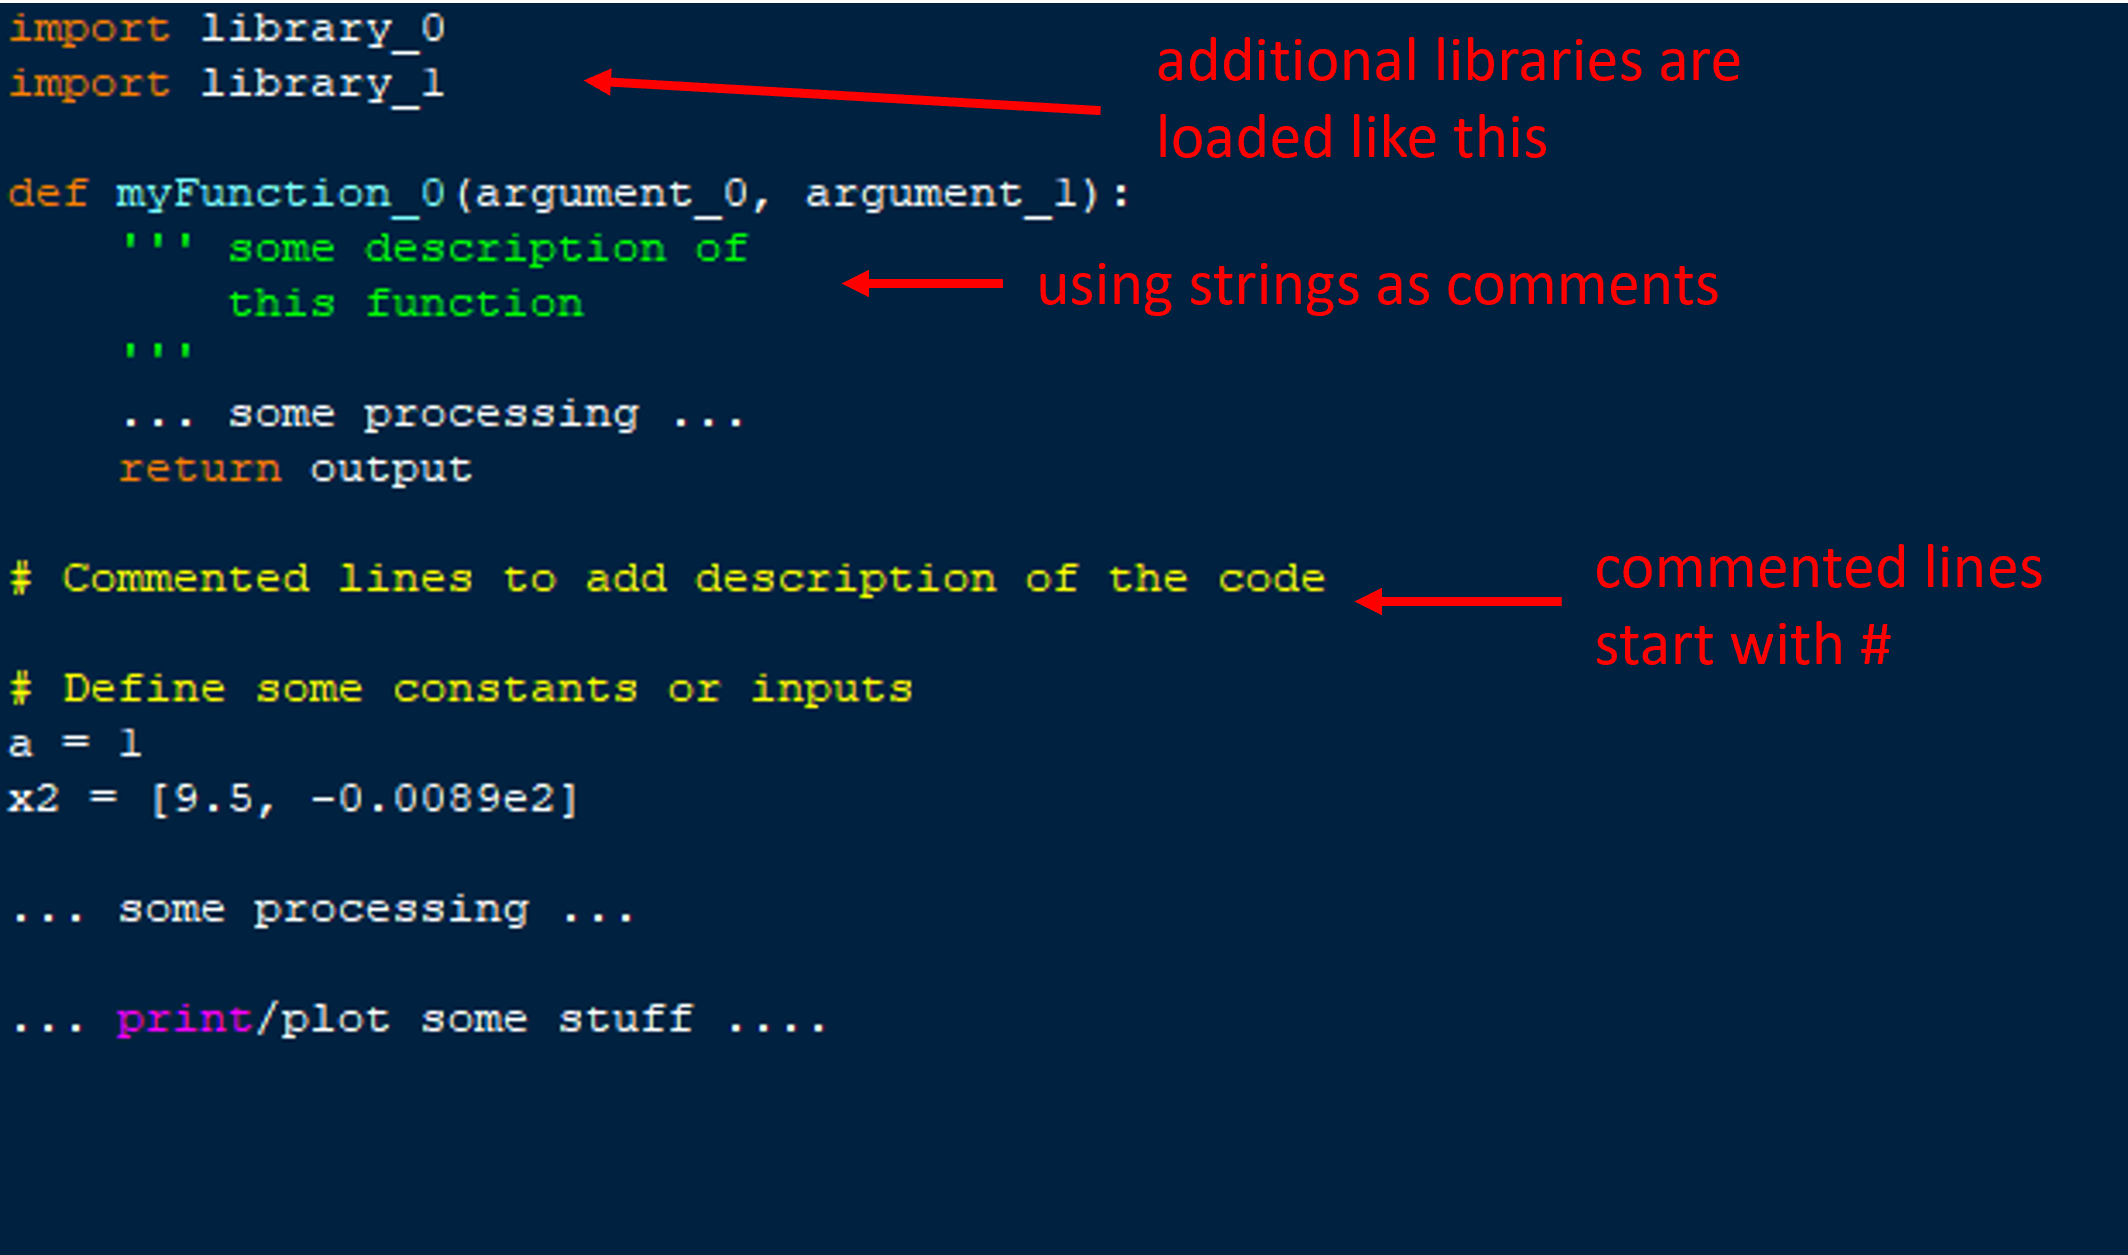
\includegraphics[width=\textwidth]{images/0_typical-code.png}
\end{figure}
\end{frame}

\begin{frame}[fragile]
\frametitle{Hello World}
Write a code that simply prints a greeting.
\begin{python}
print("Hello World...")
print()    # this will leave a blank-line in output

print('''Hello Universe...
This is my first Python code and I'm already
using a multi-line docstring, because.. why not!
''')
\end{python}
\end{frame}

\begin{frame}[fragile]
\frametitle{Find Means}
Write a code to print arithmetic mean $AM$, geometric mean $GM$ and harmonic mean $HM$ of two positive numbers. Also print $AM\times HM$ and $GM^2$.
\begin{python}
import math

a = float(input('Enter first number... '))
b = float(input('Enter second number... '))

am = (a + b) * 0.5
gm = math.sqrt(a * b)
hm = 2.0 * a * b / (a + b)

print('Their arithmetic mean AM is...', am)
print('Their geometric mean GM is...', gm)
print('Their harmonic mean HM is...', hm)
print('AM * HM =', am * hm)
print('GM * GM =', gm * gm)
\end{python}
\end{frame}

\begin{frame}[fragile]
\frametitle{Power and Left Shift Operations}
Given a non-negative \lstinline{int} $x$, write a code to print $2^x+2^{x+1}$. Also print result of applying left-shift of $x$ to $3$.
\begin{python}
x = 7
print(2**x + 2**(x+1))
print(3 << x)
\end{python}
I encourage you to repeat this for different $x$ and explain your observations.
\end{frame}

\begin{frame}[fragile]
\frametitle{Evaluate and check equation}
Given 2 numbers $z_0, z_1$, write a code to print $(z_0+z_1)^2$ and $z_0^2+2z_0 z_1+z_1^2$. Print if they match.
\begin{python}
z0 = 2.0
z1 = 3.0

lhs = (z0 + z1)**2
rhs = z0**2 + 2.0*z0*z1 + z1**2

print('1st expression:', lhs)
print('2nd expression:', rhs)
print('Equality Check:', lhs == rhs)
\end{python}
You should also try this with $z_0=2.1, z_1=3.0$ and $z_0=2.1, z_1=3.00001$.
\end{frame}

\begin{frame}[fragile]
\frametitle{Find Types}
Define a \lstinline{tuple} \pyth{t} of \pyth{5,2,2.0}. Print result and data types of \pyth{t[0] / t[1]}, \pyth{t[0] // t[1]}, \pyth{t[0] // t[2]}. Check if \pyth{t[1] == t[2]}, \pyth{t[1] is t[2]} and whether \pyth{5.0+0.0j} is in \pyth{t}.
\begin{python}
t = (5, 2, 2.0)
print(t[0] / t[1], type(t[0] / t[1]))
print(t[0] // t[1], type(t[0] // t[1]))
print(t[0] // t[2], type(t[0] // t[2]))
print(t[1] == t[2])
print(t[1] is t[2])
print(5.0+0.0j in t)
\end{python}
\end{frame}

\begin{frame}[fragile]
\frametitle{\lstinline{list} and \lstinline{dict} example}
Define a \lstinline{dict} \pyth{d} mapping \pyth{1} with \pyth{'one'} and \pyth{2} with \pyth{'two'}. Define a \lstinline{list} \pyth{q} with elements \pyth{3,4,5}. Convert \pyth{d} to another \lstinline{list} \pyth{p} using \pyth{list} command. Add the \lstinline{lists} \pyth{p} and \pyth{q} and assign the result to a variable \pyth{r}. Print \pyth{d, p, q, r} and check if \lstinline{list} \pyth{[2, 3]} is in \pyth{r}.
\begin{python}
d = {1: 'one', 2: 'two'}
q = [3, 4, 5]

p = list(d)
r = p + q

print('d =', d)
print('p =', p)
print('q =', q)
print('r =', r)
print([2, 3] in r)
\end{python}
\end{frame}

\section{Jupyter}

\begin{frame}
\frametitle{JupyterLab}
\begin{enumerate}
\item \textbf{Jupyter Lab} is a web-browser based notebook interface for python.
\item It locally runs in a web-browser and doesn't need internet connection.
\item It is very useful for data analysis kind of projects.
\item To install it in existing python environment, use \lstinline{pip install jupyterlab}.
\item Launch the Jupyter Lab using \lstinline{jupyter lab} from command prompt (or terminal).
\item It save files in \lstinline{.ipynb} format and supports markdown language.
\end{enumerate}
\end{frame}

\end{document}
